% Template for PLoS
% Version 3.5 March 2018
%
% % % % % % % % % % % % % % % % % % % % % %
%
% -- IMPORTANT NOTE
%
% This template contains comments intended
% to minimize problems and delays during our production
% process. Please follow the template instructions
% whenever possible.
%
% % % % % % % % % % % % % % % % % % % % % % %
%
% Once your paper is accepted for publication,
% PLEASE REMOVE ALL TRACKED CHANGES in this file
% and leave only the final text of your manuscript.
% PLOS recommends the use of latexdiff to track changes during review, as this will help to maintain a clean tex file.
% Visit https://www.ctan.org/pkg/latexdiff?lang=en for info or contact us at latex@plos.org.
%
%
% There are no restrictions on package use within the LaTeX files except that
% no packages listed in the template may be deleted.
%
% Please do not include colors or graphics in the text.
%
% The manuscript LaTeX source should be contained within a single file (do not use \input, \externaldocument, or similar commands).
%
% % % % % % % % % % % % % % % % % % % % % % %
%
% -- FIGURES AND TABLES
%
% Please include tables/figure captions directly after the paragraph where they are first cited in the text.
%
% DO NOT INCLUDE GRAPHICS IN YOUR MANUSCRIPT
% - Figures should be uploaded separately from your manuscript file.
% - Figures generated using LaTeX should be extracted and removed from the PDF before submission.
% - Figures containing multiple panels/subfigures must be combined into one image file before submission.
% For figure citations, please use "Fig" instead of "Figure".
% See http://journals.plos.org/plosone/s/figures for PLOS figure guidelines.
%
% Tables should be cell-based and may not contain:
% - spacing/line breaks within cells to alter layout or alignment
% - do not nest tabular environments (no tabular environments within tabular environments)
% - no graphics or colored text (cell background color/shading OK)
% See http://journals.plos.org/plosone/s/tables for table guidelines.
%
% For tables that exceed the width of the text column, use the adjustwidth environment as illustrated in the example table in text below.
%
% % % % % % % % % % % % % % % % % % % % % % % %
%
% -- EQUATIONS, MATH SYMBOLS, SUBSCRIPTS, AND SUPERSCRIPTS
%
% IMPORTANT
% Below are a few tips to help format your equations and other special characters according to our specifications. For more tips to help reduce the possibility of formatting errors during conversion, please see our LaTeX guidelines at http://journals.plos.org/plosone/s/latex
%
% For inline equations, please be sure to include all portions of an equation in the math environment.
%
% Do not include text that is not math in the math environment.
%
% Please add line breaks to long display equations when possible in order to fit size of the column.
%
% For inline equations, please do not include punctuation (commas, etc) within the math environment unless this is part of the equation.
%
% When adding superscript or subscripts outside of brackets/braces, please group using {}.
%
% Do not use \cal for caligraphic font.  Instead, use \mathcal{}
%
% % % % % % % % % % % % % % % % % % % % % % % %
%
% Please contact latex@plos.org with any questions.
%
% % % % % % % % % % % % % % % % % % % % % % % %

\documentclass[10pt,letterpaper]{article}
\usepackage[top=0.85in,left=2.75in,footskip=0.75in]{geometry}

% amsmath and amssymb packages, useful for mathematical formulas and symbols
\usepackage{amsmath,amssymb}

% Use adjustwidth environment to exceed column width (see example table in text)
\usepackage{changepage}

% Use Unicode characters when possible
\usepackage[utf8x]{inputenc}

% textcomp package and marvosym package for additional characters
\usepackage{textcomp,marvosym}

% cite package, to clean up citations in the main text. Do not remove.
% \usepackage{cite}

% Use nameref to cite supporting information files (see Supporting Information section for more info)
\usepackage{nameref,hyperref}

% line numbers
\usepackage[right]{lineno}

% ligatures disabled
\usepackage{microtype}
\DisableLigatures[f]{encoding = *, family = * }

% color can be used to apply background shading to table cells only
\usepackage[table]{xcolor}

% array package and thick rules for tables
\usepackage{array}

% create "+" rule type for thick vertical lines
\newcolumntype{+}{!{\vrule width 2pt}}

% create \thickcline for thick horizontal lines of variable length
\newlength\savedwidth
\newcommand\thickcline[1]{%
  \noalign{\global\savedwidth\arrayrulewidth\global\arrayrulewidth 2pt}%
  \cline{#1}%
  \noalign{\vskip\arrayrulewidth}%
  \noalign{\global\arrayrulewidth\savedwidth}%
}

% \thickhline command for thick horizontal lines that span the table
\newcommand\thickhline{\noalign{\global\savedwidth\arrayrulewidth\global\arrayrulewidth 2pt}%
\hline
\noalign{\global\arrayrulewidth\savedwidth}}


% Remove comment for double spacing
%\usepackage{setspace}
%\doublespacing

% Text layout
\raggedright
\setlength{\parindent}{0.5cm}
\textwidth 5.25in
\textheight 8.75in

% Bold the 'Figure #' in the caption and separate it from the title/caption with a period
% Captions will be left justified
\usepackage[aboveskip=1pt,labelfont=bf,labelsep=period,justification=raggedright,singlelinecheck=off]{caption}
\renewcommand{\figurename}{Fig}

% Use the PLoS provided BiBTeX style
% \bibliographystyle{plos2015}

% Remove brackets from numbering in List of References
\makeatletter
\renewcommand{\@biblabel}[1]{\quad#1.}
\makeatother



% Header and Footer with logo
\usepackage{lastpage,fancyhdr,graphicx}
\usepackage{epstopdf}
%\pagestyle{myheadings}
\pagestyle{fancy}
\fancyhf{}
%\setlength{\headheight}{27.023pt}
%\lhead{
\includegraphics[width=2.0in]{PLOS-submission.eps}}
\rfoot{\thepage/\pageref{LastPage}}
\renewcommand{\headrulewidth}{0pt}
\renewcommand{\footrule}{\hrule height 2pt \vspace{2mm}}
\fancyheadoffset[L]{2.25in}
\fancyfootoffset[L]{2.25in}
\lfoot{\today}

%% Include all macros below

\newcommand{\lorem}{{\bf LOREM}}
\newcommand{\ipsum}{{\bf IPSUM}}

\usepackage{color}
\usepackage{fancyvrb}
\newcommand{\VerbBar}{|}
\newcommand{\VERB}{\Verb[commandchars=\\\{\}]}
\DefineVerbatimEnvironment{Highlighting}{Verbatim}{commandchars=\\\{\}}
% Add ',fontsize=\small' for more characters per line
\usepackage{framed}
\definecolor{shadecolor}{RGB}{248,248,248}
\newenvironment{Shaded}{\begin{snugshade}}{\end{snugshade}}
\newcommand{\AlertTok}[1]{\textcolor[rgb]{0.94,0.16,0.16}{#1}}
\newcommand{\AnnotationTok}[1]{\textcolor[rgb]{0.56,0.35,0.01}{\textbf{\textit{#1}}}}
\newcommand{\AttributeTok}[1]{\textcolor[rgb]{0.77,0.63,0.00}{#1}}
\newcommand{\BaseNTok}[1]{\textcolor[rgb]{0.00,0.00,0.81}{#1}}
\newcommand{\BuiltInTok}[1]{#1}
\newcommand{\CharTok}[1]{\textcolor[rgb]{0.31,0.60,0.02}{#1}}
\newcommand{\CommentTok}[1]{\textcolor[rgb]{0.56,0.35,0.01}{\textit{#1}}}
\newcommand{\CommentVarTok}[1]{\textcolor[rgb]{0.56,0.35,0.01}{\textbf{\textit{#1}}}}
\newcommand{\ConstantTok}[1]{\textcolor[rgb]{0.00,0.00,0.00}{#1}}
\newcommand{\ControlFlowTok}[1]{\textcolor[rgb]{0.13,0.29,0.53}{\textbf{#1}}}
\newcommand{\DataTypeTok}[1]{\textcolor[rgb]{0.13,0.29,0.53}{#1}}
\newcommand{\DecValTok}[1]{\textcolor[rgb]{0.00,0.00,0.81}{#1}}
\newcommand{\DocumentationTok}[1]{\textcolor[rgb]{0.56,0.35,0.01}{\textbf{\textit{#1}}}}
\newcommand{\ErrorTok}[1]{\textcolor[rgb]{0.64,0.00,0.00}{\textbf{#1}}}
\newcommand{\ExtensionTok}[1]{#1}
\newcommand{\FloatTok}[1]{\textcolor[rgb]{0.00,0.00,0.81}{#1}}
\newcommand{\FunctionTok}[1]{\textcolor[rgb]{0.00,0.00,0.00}{#1}}
\newcommand{\ImportTok}[1]{#1}
\newcommand{\InformationTok}[1]{\textcolor[rgb]{0.56,0.35,0.01}{\textbf{\textit{#1}}}}
\newcommand{\KeywordTok}[1]{\textcolor[rgb]{0.13,0.29,0.53}{\textbf{#1}}}
\newcommand{\NormalTok}[1]{#1}
\newcommand{\OperatorTok}[1]{\textcolor[rgb]{0.81,0.36,0.00}{\textbf{#1}}}
\newcommand{\OtherTok}[1]{\textcolor[rgb]{0.56,0.35,0.01}{#1}}
\newcommand{\PreprocessorTok}[1]{\textcolor[rgb]{0.56,0.35,0.01}{\textit{#1}}}
\newcommand{\RegionMarkerTok}[1]{#1}
\newcommand{\SpecialCharTok}[1]{\textcolor[rgb]{0.00,0.00,0.00}{#1}}
\newcommand{\SpecialStringTok}[1]{\textcolor[rgb]{0.31,0.60,0.02}{#1}}
\newcommand{\StringTok}[1]{\textcolor[rgb]{0.31,0.60,0.02}{#1}}
\newcommand{\VariableTok}[1]{\textcolor[rgb]{0.00,0.00,0.00}{#1}}
\newcommand{\VerbatimStringTok}[1]{\textcolor[rgb]{0.31,0.60,0.02}{#1}}
\newcommand{\WarningTok}[1]{\textcolor[rgb]{0.56,0.35,0.01}{\textbf{\textit{#1}}}}


\usepackage[T1]{fontenc}
\usepackage{lmodern}
\usepackage[user,titleref]{zref}
\usepackage{nameref}
\newcommand*{\rulelabel}[2]{\ztitlerefsetup{title=#1} \zlabel{#2} \label{#2} \zrefused{#2}}
\newcommand*{\ruleref}[1]{\hyperref[{#1}]{Rule~\ztitleref{#1}}}
\usepackage{listings}
\lstdefinelanguage{docker}{keywords={FROM, RUN, COPY, ADD, ENTRYPOINT, CMD,  ENV, ARG, WORKDIR, EXPOSE, LABEL, USER, VOLUME, STOPSIGNAL, ONBUILD, MAINTAINER}, keywordstyle=\color{blue}\bfseries, identifierstyle=\color{black}, sensitive=false, comment=[l]{\#}, commentstyle=\color{darkgray}\ttfamily, stringstyle=\color{red}\ttfamily, morestring=[b]', morestring=[b]"}
\lstset{literate={ü}{{\"u}}1, showstringspaces=false}



\usepackage{forarray}
\usepackage{xstring}
\newcommand{\getIndex}[2]{
  \ForEach{,}{\IfEq{#1}{\thislevelitem}{\number\thislevelcount\ExitForEach}{}}{#2}
}

\setcounter{secnumdepth}{0}

\newcommand{\getAff}[1]{
  \getIndex{#1}{}
}

\providecommand{\tightlist}{%
  \setlength{\itemsep}{0pt}\setlength{\parskip}{0pt}}

\begin{document}
\vspace*{0.2in}

% Title must be 250 characters or less.
\begin{flushleft}
{\Large
\textbf\newline{Ten Simple Rules for Writing Dockerfiles for Reproducible Data Science} % Please use "sentence case" for title and headings (capitalize only the first word in a title (or heading), the first word in a subtitle (or subheading), and any proper nouns).
}
\newline
% Insert author names, affiliations and corresponding author email (do not include titles, positions, or degrees).
\\
Daniel Nüst\textsuperscript{\getAff{Institute for Geoinformatics, University of Muenster, Muenster, Germany}}\textsuperscript{*},
Vanessa Sochat\textsuperscript{\getAff{Stanford Research Computing Center, Stanford University, Stanford, CA,
USA}},
Ben Marwick\textsuperscript{\getAff{Department of Anthropology, University of Washington, Seattle, WA, USA}},
Stephen J. Eglen\textsuperscript{\getAff{Department of Applied Mathematics and Theoretical Physics, University of
Cambridge, Cambridge, Cambridgeshire, GB}},
Tim Head\textsuperscript{\getAff{Wild Tree Tech, Zurich, CH}},
Tony Hirst\textsuperscript{\getAff{Department of Computing and Communications, The Open University, GB}},
Benjamin D. Evans\textsuperscript{\getAff{School of Psychological Science, University of Bristol, Bristol, GB}}\\
\bigskip
\bigskip
* Corresponding author: daniel.nuest@uni-muenster.de\\
\end{flushleft}
% Please keep the abstract below 300 words
\section*{Abstract}
Computational science has been greatly improved by containers, which can
package software and data dependencies. In a scholarly context, the main
drivers for using these containers are transparency and support of
reproducibility; in turn, a workflow's reproducibility can be greatly
affected by the choices that are made with respect to building
containers. Because the build for the container's image is often created
based on the instructions in the \texttt{Dockerfile} format, here we
present rules to help researchers write understandable
\texttt{Dockerfile}s for typical data science workflows. By following
the rules in this article, researchers can create containers suitable
for sharing with fellow scientists, for including in scholarly
communication such as education or scientific papers, and for effective
and sustainable personal workflows.

% Please keep the Author Summary between 150 and 200 words
% Use first person. PLOS ONE authors please skip this step.
% Author Summary not valid for PLOS ONE submissions.
\section*{Author summary}
Computers and algorithms are ubiquitous in research. Therefore, defining
the computing environment, i.e., the body of all software used directly
or indirectly by a researcher, is important, because it allows other
researchers to recreate the environment to understand, inspect, and
reproduce an analysis. A helpful abstraction for capturing the computing
environment is a \emph{container}, whereby a container is created from a
set of instructions in a recipe. For the most common containerisation
software, Docker, this recipe is called a Dockerfile. We think that in a
scientific context, researchers should follow specific practices for
writing a Dockerfile, and these practices might be somewhat different
from the practices of generic software developers in that researchers
should focus on transparency and understandability over performance
considerations. The rules presented here are intended to help
researchers, especially newcomers to containerisation, leverage
containers for open and effective scholarly communication and
collaboration while avoiding the pitfalls that are especially irksome in
a research lifecycle. The recommendations cover a deliberate approach to
Dockerfile creation, formatting and style, documentation, and habits for
using containers.

\linenumbers

% Use "Eq" instead of "Equation" for equation citations.
\hypertarget{introduction}{%
\section*{Introduction}\label{introduction}}
\addcontentsline{toc}{section}{Introduction}

Computing infrastructure has advanced to the point where not only can we
share data underlying research articles, but we can also share the code
that processes these data. This sharing of code files is enabled by
collaboration platforms such as \href{https://github.com}{GitHub} or
\href{https://gitlab.com}{GitLab} and has become quite common. The
sharing of the computing environment, on the other hand, is enabled by
containerisation, which allows for documenting and sharing entire
workflows in a comprehensive way. Importantly, this sharing of
computational assets is paramount for increasing the reproducibility of
computational research. While papers based on the traditional journal
article format can share extensive details about the research,
computational research is often far too complicated to be effectively
disseminated in this format {[}1{]}. In this field and whenever software
is used to analyse or visualise data, containerisation is needed because
a papers's actual contribution to knowledge includes the full computing
environment that produced a result {[}2{]}.

Containerisation helps provide instructions for packaging the building
blocks of computer-based research (i.e., code, data, documentation, and
the computing environment). Specifically, containers are built from
plain text files (via an image) that represent a human- \emph{and}
machine-readable recipe for creating the computing environment and
interacting with data. By providing this recipe, authors of scientific
articles greatly improve their work's level of documentation,
transparency, and reusability, which is an important part of common
practices for scientific computing {[}3,4{]}; an overall goal of these
practices is to ensure that both the author and others are able to
reproduce and extend an analysis workflow. The containers built from
these recipes are portable encapsulated snapshots of a specific
computing environment that are both more lightweight and transparent
than virtual machines. Such containers have been demonstrated for
capturing scientific notebooks {[}5{]} and reproducible workflows
{[}6{]}.

While several tutorials exist on how to use containers for reproducible
research ({[}7--11{]} and Guening et~al. {[}12{]} give very helpful
recommendations for packaging reusable software in a container), there
is no detailed \emph{manual for how to write the actual instructions to
create the containers for computational research} besides generic best
practices {[}13,14{]}. Here we introduce these instructions for the
popular \texttt{Dockerfile} format in the context of data science
workflows, summarised in Figure~\ref{fig:summary}.

\begin{figure}[h]
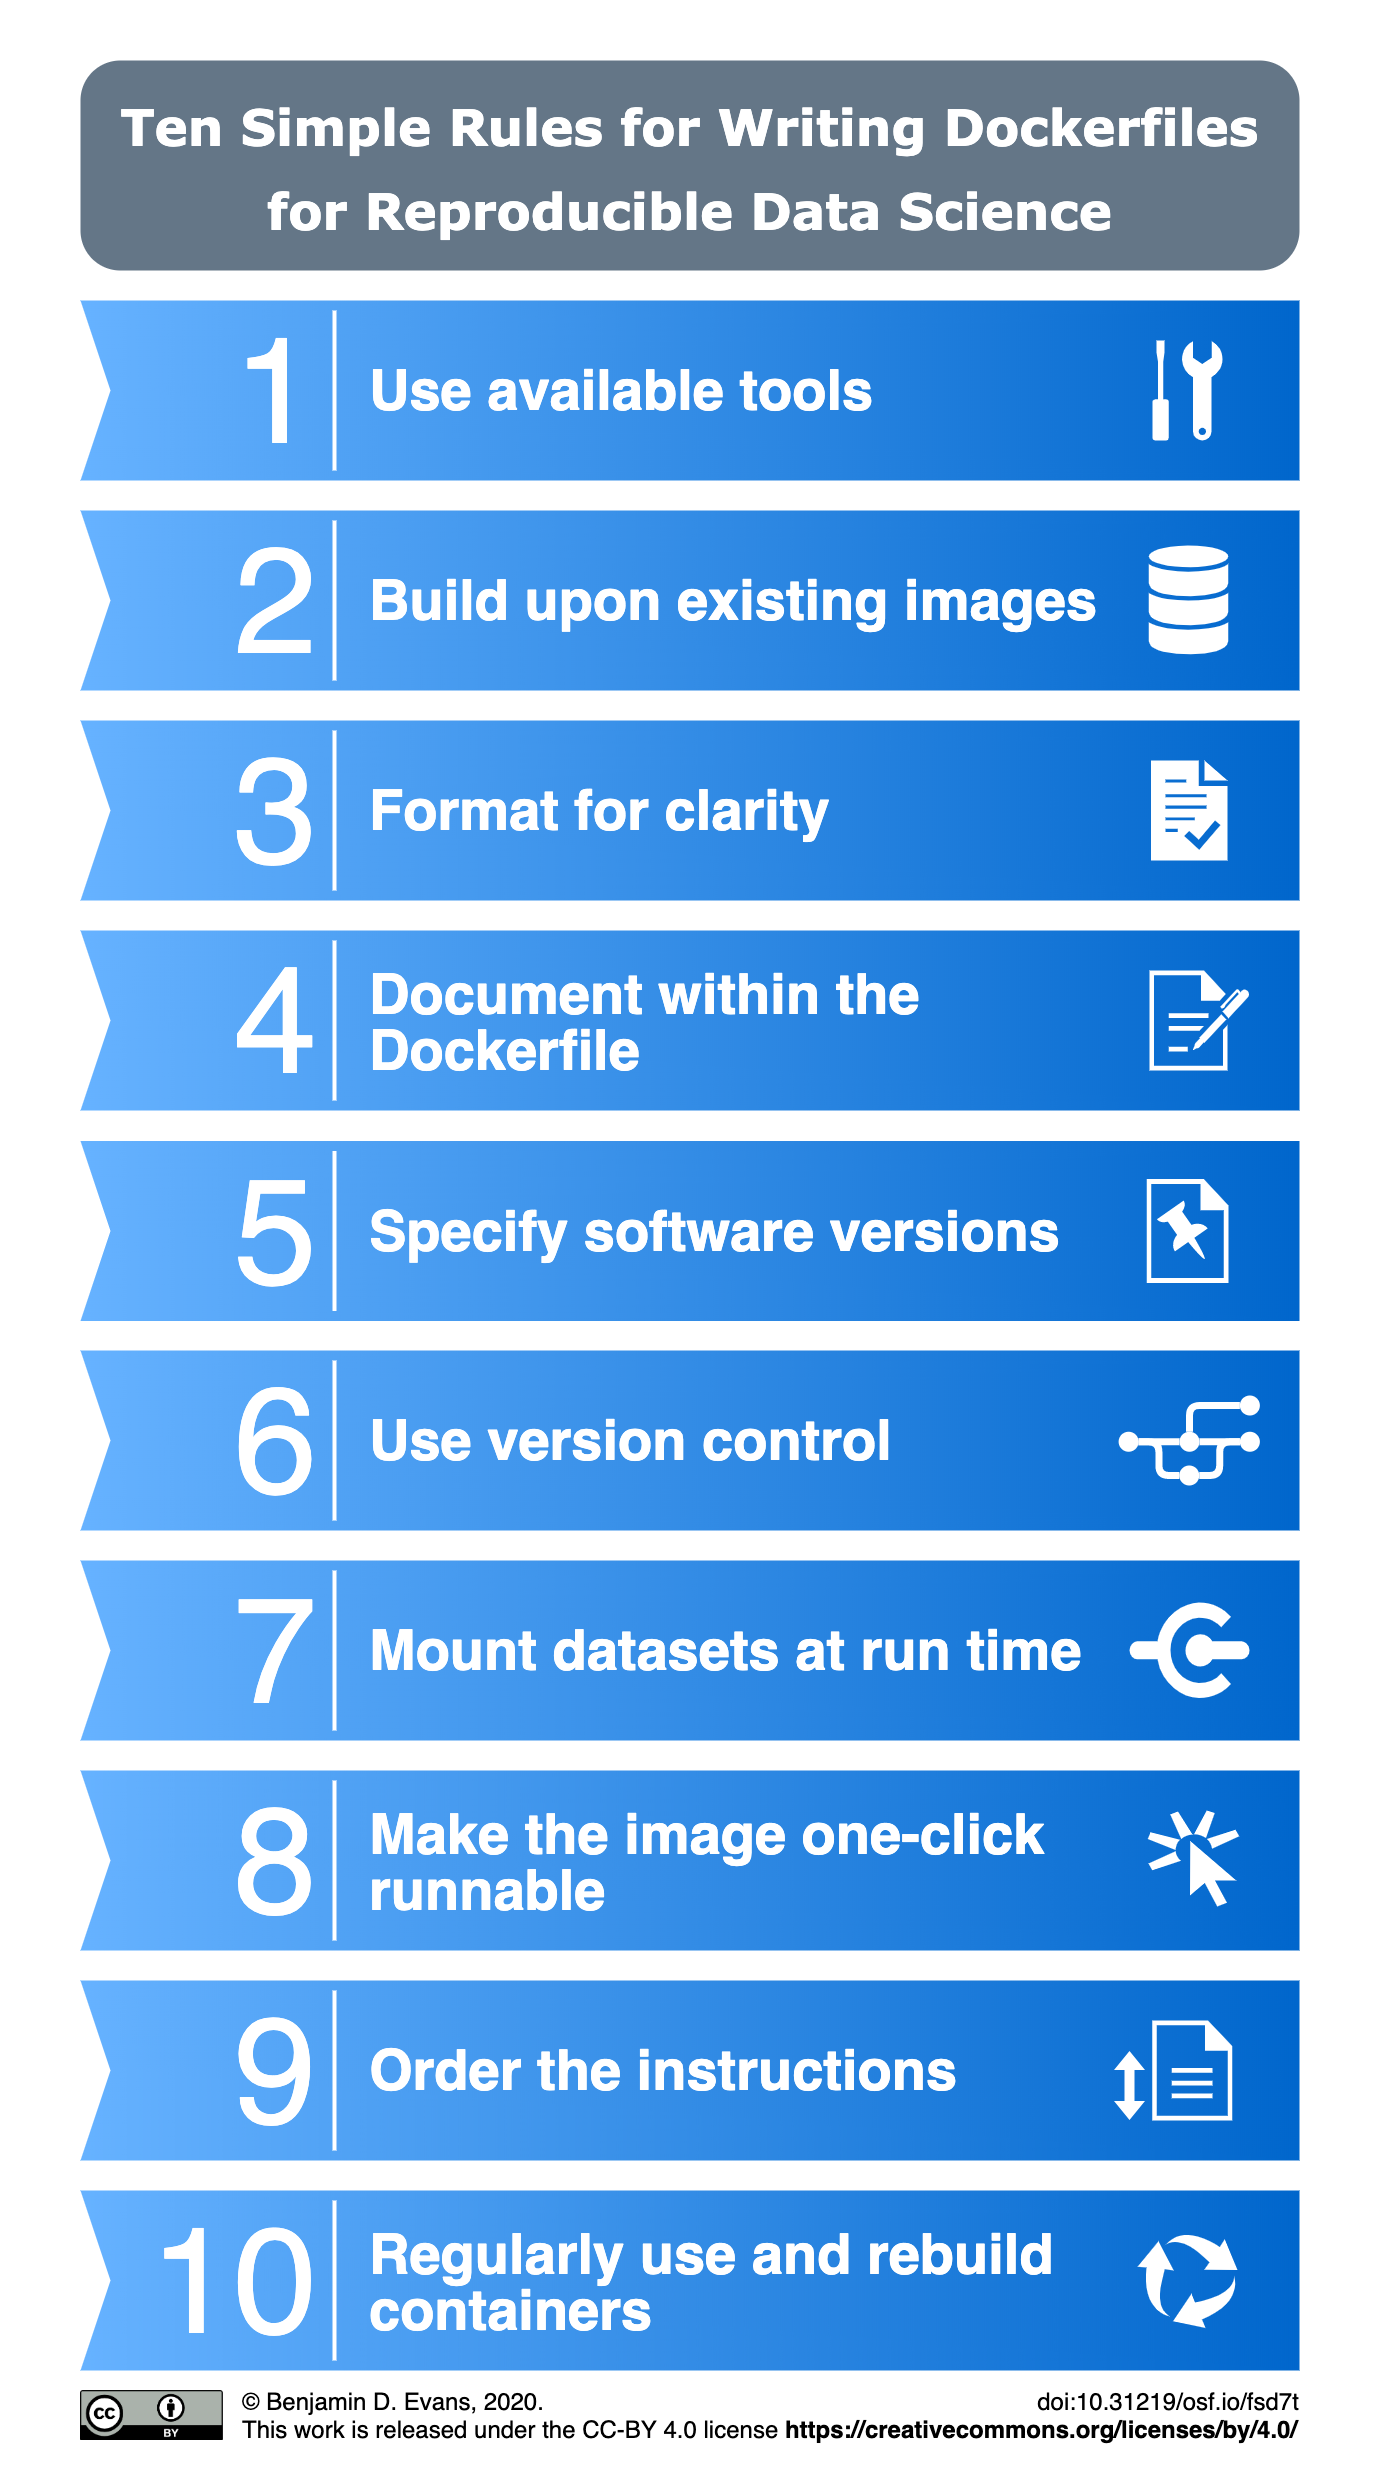
\includegraphics[width=0.5\linewidth]{summary} \caption{Summary of the ten simple rules for writing \texttt{Dockerfile}s for reproducible data science.}\label{fig:summary}
\end{figure}

\hypertarget{prerequisites-scope}{%
\section{Prerequisites \& scope}\label{prerequisites-scope}}

To start with, we assume you have a scripted scientific workflow,
i.e.~you can, at least at a certain point in time, execute the full
process with a fixed set of commands, for example
\texttt{make\ prepare\_data} followed by \texttt{Rscript\ analysis.R},
or only \texttt{python3\ my-workflow.py}. Since containers that you
eventually share with others can only run open source software, tools
like Mathematica and Matlab are out of scope for this example. A
workflow that does not support scripted execution is also out of scope
for reproducible research, as it does not fit well with
containerisation. Furthermore, workflows interacting with many petabytes
of data and executed in high-performance computing (HPC) infrastructures
are out of scope. Using such HPC job managers or cloud infrastructures
would require a collection of ``Ten Simple Rules'' articles in their own
right. For the HPC use case, we encourage the reader to look at
Singularity {[}15{]}. For this article, we focus on workflows that
typically run on single machine, e.g., a researchers laptop computer or
a virtual server. The reader might scope the data requirement to under a
terabyte, and compute requirement to a machine with 16 cores running
over the weekend.

Although it is outside the scope of this article, we point readers to
\texttt{docker-compose} {[}16{]} in the case where one might need
container orchestration for multiple applications, e.g., web servers,
databases, and worker containers. A \texttt{docker-compose.yml}
configuration file allows for defining mounts, environment variables,
and exposed ports and helps users stick to \emph{one purpose per
container}, which often means one process running in the container, and
to combine existing stable building blocks instead of bespoke massive
containers for specific purposes.

Because \emph{``the number of unique research environments approximates
the number of researchers''} {[}17{]}, sticking to conventions helps
every researcher to understand, modify, and eventually write container
recipes suitable for their needs. Even if they are not sure how the
underlying technology actually works, researchers should leverage
containerisation following good practices. The practices that are to be
discussed in this article are strongly related to software engineering
in general and research software engineering in particular, which is
concerned with quality, training, and recognition of software in science
{[}18{]}. We encourage you to reach out to your local or national
community of research software engineers (see
\href{https://en.wikipedia.org/wiki/Research_software_engineering}{list
of organisations}) if you have questions on software development in
research that go beyond the rules of this work.

While many different container technologies exist, this article focuses
on Docker {[}19{]}. Docker is a highly suitable tool for reproducible
research (e.g., {[}20{]}), and our observations indicate it is the most
widely used container technology in academic data science. The goal of
this article is to guide you as you write a \texttt{Dockerfile}, which
is a file format for creating container images. The rules will help you
ensure that the \texttt{Dockerfile} allows for interactive development
as well as for reaching the higher goals of reproducibility and
preservation of knowledge. Such practices are generally not part of
generic containerisation tutorials and are rarely found in
\texttt{Dockerfile}s published as part of software projects that are
often used as templates by novices. The differences between a helpful,
stable \texttt{Dockerfile} and one that is misleading, prone to failure,
and full of potential obstacles are not obvious, especially for
researchers who do not have extensive software development experience or
formal training. Yet, by committing to this article's rules, one can
ensure that their workflows are reproducible and reusable, that
computing environments are understandable by others, and that
researchers have the opportunity to collaborate effectively. Applying
these rules should not be triggered by the publication of a finished
project but should instead be weaved into day-to-day habits
(cf.~thoughts on openness as an afterthought by {[}21{]} and on
computational reproducibility by {[}2{]}).

\hypertarget{docker-dockerfiles}{%
\section{Docker \& Dockerfiles}\label{docker-dockerfiles}}

Docker {[}19{]} is a container technology that has been widely adopted
and is supported on many platforms, and it has become highly useful for
research. Containers are distinct from virtual machines or hypervisors,
as they do not emulate hardware or operating system kernels and, thus,
do not require the same system resources. Several solutions for
facilitating reproducible research are built on top of containers
{[}17,22--25{]}, but these solutions intentionally hide most of the
complexity from the researcher.

To create Docker containers for specific workflows, we write text files
that follow a particular format called \texttt{Dockerfile} {[}26{]},
whereby a \texttt{Dockerfile} is a machine- \emph{and} human-readable
recipe for building images, comparable to a \texttt{Makefile} {[}27{]}.
Here, container images include the application, e.g., the programming
language interpreter needed to run a workflow, and the system libraries
required by an application to run. Thus, a \texttt{Dockerfile} consists
of a sequence of instructions to copy files and install software. Each
instruction adds a layer to the image, which can be cached across image
builds for minimizing build and download times. The images have a main
executable exposed as an ``entrypoint'' that is started when they are
run as stateful containers, which are the running instances of Docker
images. Further, containers can be modified, stopped, restarted and
purged.

A visual analogy for building and running a container is provided in
Figure~\ref{fig:analogy}. Akin to compiling source code for a
programming language, creating a container also starts with a plain text
file (\texttt{Dockerfile}), which provides instructions for building an
image. Similar to using a compiled binary file to launch a program, the
image is then run to create a container instance. See
Listing~\ref{lst:full} for a full \texttt{Dockerfile}, which we will
refer to throughout this article.

\begin{figure}[h]
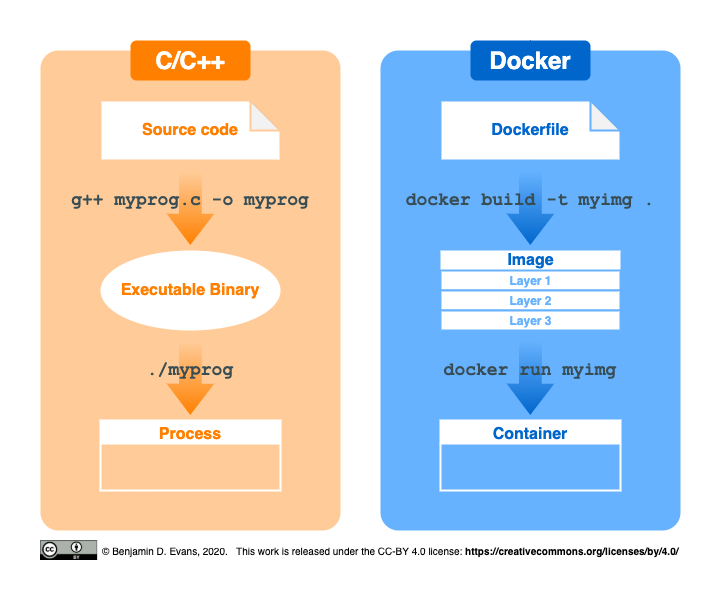
\includegraphics[width=1\linewidth]{analogy} \caption{The workflow to create Docker containers by analogy. Containers begin with a \texttt{Dockerfile}, a recipe for building the computational environment (analogous to source code in a compiled programming language). This is used to build an image with the \texttt{docker build} command, analogous to compiling the source code into an executable (binary) file. Finally, the image is used to launch one or more containers with the \texttt{docker run} command (analogous to running an instance of the compiled binary as a process).}\label{fig:analogy}
\end{figure}

While Docker was the original technology to support the
\texttt{Dockerfile} format, other container technologies with support
include
\href{https://podman.io/}{podman}/\href{https://github.com/containers/buildah}{buildah}
supported by RedHat,
\href{https://github.com/GoogleContainerTools/kaniko}{kaniko},
\href{https://github.com/genuinetools/img}{img}, and
\href{https://github.com/moby/buildkit}{buildkit}. The container
software Singularity {[}15{]}, which is optimised for scientific
computing and the security needs of HPC environments, uses its own
format, called the \emph{Singularity recipe}, but it can also import and
run Docker images. The rules here are transferable to Singularity
recipes to some extent.

While some may argue against publishing reproducibly, e.g., due to a
lack of time and incentives, a reluctance to share (cf.~{[}28{]}), and
the substantial technical challenges involved in maintaining software
and documentation, it should become increasingly easier for the average
researcher to provide with their publication a \texttt{Dockerfile}, a
pre-built Docker image, or another type of container. If a researcher
can find and create containers or write a \texttt{Dockerfile} to address
their most common use cases, then, arguably, providing it would not make
for extra work after this initial setup (cf.~\texttt{README.md} of
{[}29{]}). In fact, the \texttt{Dockerfile} itself represents powerful
documentation to show from where data and code were derived, i.e.,
downloaded or installed, and, consequently, where a third party might
obtain the data again.

\clearpage

\scriptsize

\begin{lstlisting}[language=docker,caption={\texttt{Dockerfile} full example. The \texttt{Dockerfile} and all other files are published in the \texttt{full-demo} example, see Section~\nameref{examples}; the image \texttt{nuest/datascidockerfiles:1.0.0} is a ready-to-use build of this example.},breaklines=true,label={lst:full}]

FROM docker.io/rocker/verse:3.6.2

### INSTALL BASE SOFTWARE #####################################################
# Install Java, needed for package rJava
RUN apt-get update && \
  apt-get install -y default-jdk && \
  rm -rf /var/lib/apt/lists/*

### INSTALL WORKFLOW TOOLS ####################################################
# Install system dependencies for R packages
RUN apt-get update && \
  apt-get install -y \
    # needed for RNetCDF, found via https://sysreqs.r-hub.io/pkg/RNetCDF
    libnetcdf-dev libudunits2-dev \
    # needed for git2r:
    libgit2-dev

# Install R packages, based on https://github.com/rocker-org/geospatial/blob/master/Dockerfile
RUN install2.r --error \
    RColorBrewer \
    RNetCDF \
    git2r \
    rJava

WORKDIR /tmp

# Install Python tools and their system dependencies
RUN apt-get update && \
  apt-get install -y python-pip && \
  rm -rf /var/lib/apt/lists/*
COPY requirements.txt requirements.txt
RUN pip install -r requirements.txt

# Download superduper image converter
RUN wget https://downloads.apache.org/pdfbox/2.0.19/pdfbox-app-2.0.19.jar

### ADD MY OWN SCRIPTS ########################################################
# Add workflow scripts
WORKDIR /work
COPY myscript.sh myscript.sh
COPY analysis.py analysis.py
COPY plots.R plots.R

# Configure workflow
ENV DATA_SIZE 42

# Uncomment the following lines to execute preprocessing tasks during build
#RUN python analysis.py
#RUN Rscript plots.R

### WORKFLOW CONTAINER FEATURE ################################################
# CMD from base image used for development, uncomment the following lines to 
# have a "run workflow only" image
# CMD["./myscript.sh"]

### Usage instructions ########################################################
# Build the images with
# > docker build --tag datascidockerfiles:1.0.0 .
# Run the image interactively with RStudio, open it on http://localhost/
# > docker run -it -p 80:8787 -e PASSWORD=ten --volume $(pwd)/input:/input datascidockerfiles:1.0.0
# Run the workflow:
# > docker run -it --name gwf datascidockerfiles:1.0.0 /work/myscript.sh
# Extract the data:
# > docker cp gwf:/output/ ./outputData
# Extract the figures:
# > docker cp gwf:/work/figures/ ./figures

\end{lstlisting}

\normalsize

\newpage

\hypertarget{use-available-tools}{%
\section*{1. Use available tools}\label{use-available-tools}}
\addcontentsline{toc}{section}{1. Use available tools}

\ztitlerefsetup{title=1} \zlabel{rule:tools} \label{rule:tools} \zrefused{rule:tools}

Rule 1 could informally be described as ``Don't bother to write a
Dockerfile!''. Writing a \texttt{Dockerfile} from scratch can be
difficult, and even experts sometimes take shortcuts. Thus, a good
strategy is to first look at tools that can help generate a
\texttt{Dockerfile} for you. Such tools have likely thought about and
implemented good practices, and they may even have incorporated newer
practices when reapplied at a later point in time. Therefore, the most
important rule is to apply a multi-step process for your specific use
case.

First, you want to determine whether there is an existing image that you
can use; if so, you want to be able to use it and add the instructions
for doing so to your workflow documentation. As an example, you might be
doing some kind of interactive development. For interactive development
environments such as notebooks and development servers or databases, you
can readily find images that come installed with all the software that
you need. You can look for information about images in (a) the
documentation of the used software, (b) the Docker image registry
\emph{Docker Hub}, \url{https://hub.docker.com/}, or (c) the source code
projects of the used software, as many developers today rely on
containers for development, testing, and teaching.

Second, if there is no suitable pre-existing image for your needs, you
might next look to well-maintained tools to help with
\texttt{Dockerfile} generation. These tools can add required software
packages to an existing image without you having to manually write a
\texttt{Dockerfile} at all. ``Well-maintained'' not only refers to the
tool's own stability and usability but also indicates that suitable base
images are used, likely from the official Docker library {[}30{]}, to
ensure that the container has the most recent security fixes for the
operating system in question. See the next section ``Tools for container
generation'' for details.

Third, if these tools do not meet your needs, you may want to write you
own \texttt{Dockerfile}. \emph{In this case, follow the remaining
rules.}

\begin{center}\rule{0.5\linewidth}{0.5pt}\end{center}

\hypertarget{tools-for-container-generation}{%
\subsection{Tools for container
generation}\label{tools-for-container-generation}}

\texttt{repo2docker} {[}25{]} is a tool maintained by
\href{https://jupyter.org/}{Project Jupyter} that can help to transform
a source code or data repository, e.g., GitHub, GitLab, or Zenodo, into
a container. The tool relies on common configuration files for defining
software dependencies and versions, and it supports a few more special
files; see the
\href{https://repo2docker.readthedocs.io/en/latest/config_files.html}{supported
configuration files}. As an example, we might install
\texttt{jupyter-repo2docker} and then run it against a repository with a
\texttt{requirements.txt} file, an indication of being a Python workflow
with dependencies on the \href{https://pypi.org/}{Python Package Index}
(PyPI), using the following command:

\footnotesize

\begin{Shaded}
\begin{Highlighting}[]
\ExtensionTok{jupyter-repo2docker}\NormalTok{ https://github.com/norvig/pytudes}
\end{Highlighting}
\end{Shaded}

\normalsize

The resulting container image installs the dependencies listed in the
requirements file, and it provides an entrypoint to run a notebook
server to interact with any existing workflows in the repository. Since
\texttt{repo2docker} is used within
\href{https://mybinder.org/}{MyBinder.org}, if you make sure your
workflow is ``Binder-ready,'' you and others can also obtain an online
workspace with a single click. However, one precaution to consider is
that the default command above will create a home for the current user,
meaning that the container itself would not be ideal to share; instead,
any researcher interested in interacting with the code inside should run
\texttt{repo2docker} themselves and create their own container. Because
\texttt{repo2docker} is deterministic, the environments are the same
(see~\hyperref[{rule:pinning}]{Rule~\ztitleref{rule:pinning}} for
ensuring the same software versions).

Additional tools to assist with writing \texttt{Dockerfile}s include
\texttt{containerit} {[}31{]} and \texttt{dockta} {[}32{]}.
\texttt{containerit} automates the generation of a standalone
\texttt{Dockerfile} for workflows in R. It can provide a starting point
for users unfamiliar with writing a \texttt{Dockerfile}, or it can,
together with other R packages, provide a full image creation and
execution process without having to leave an R session. \texttt{dockta}
supports multiple programming languages and configurations files, just
as \texttt{repo2docker} does, but it attempts to create a readable
\texttt{Dockerfile} compatible with plain Docker and to improve user
experience by cleverly adjusting instructions to reduce build time.
While perhaps more useful for fine-tuning, linters can also be helpful
when writing Dockerfiles, by catching errors or non-recommended
formulations (see \hyperref[{rule:usage}]{Rule~\ztitleref{rule:usage}}).

\hypertarget{tools-for-templating}{%
\subsection{Tools for templating}\label{tools-for-templating}}

It is likely going to be the case that over time you will work on
projects and develop images that are similar in nature to each other. To
avoid constantly repeating yourself, you should consider adopting a
standard workflow that will give you a clean slate for a new project. As
an example, cookie cutter templates {[}33{]} or community templates
(e.g., {[}34{]}) can provide the required structure and files (e.g., for
documentation, CI, and licenses), for getting started. If you decide to
build your own cookie cutter template, consider collaborating with your
community during development of the standard to ensure it will be useful
to others.

Part of your project template should be a protocol for publishing the
\texttt{Dockerfile} and even exporting the image to a suitable location,
e.g., a container registry or data repository, taking into consideration
how your workflow can receive a DOI for citation. A template is
preferable to your own set of base images because of the maintenance
efforts the base images require. Therefore, instead of building your own
independent solution, consider contributing to existing suites of images
(see \hyperref[{rule:base}]{Rule~\ztitleref{rule:base}}) and improving
these for your needs.

For any tool that you use, be sure to look at documentation for usage
and configuration options, and look for options to add metadata (e.g.,
labels see~\hyperref[{rule:document}]{Rule~\ztitleref{rule:document}}).

\begin{center}\rule{0.5\linewidth}{0.5pt}\end{center}

\hypertarget{build-upon-existing-images}{%
\section*{2. Build upon existing
images}\label{build-upon-existing-images}}
\addcontentsline{toc}{section}{2. Build upon existing images}

\ztitlerefsetup{title=2} \zlabel{rule:base} \label{rule:base} \zrefused{rule:base}

Many pre-built community and developer contributed Docker images are
publically available for anyone to pull, run and extend, without having
to replicate their construction. However, a good understanding of how
\emph{base images} and \emph{image tags} work is crucial, as the image
and tag that you choose has important implications for your derived
images and containers. It is good practice to use \textbf{base images}
that are maintained by the Docker library, so called \emph{``official
images''} {[}35{]}, which benefit from a review for best practices and
vulnerability scanning {[}13{]}. You can identify these images by the
missing user portion of the image name, which comes before the
\texttt{/}, e.g., \texttt{r-base} or \texttt{python}. However, these
images only provide basic programming languages or very widely used
software, so you will likely use images maintained by organisations or
fellow researchers.

While some organisations can be trusted to update images with security
fixes (see list below), for most individual accounts that provide
ready-to-use images, it is likely that these will not be updated
regularly. Further, it's even possible that an image or a
\texttt{Dockerfile} could disappear, or an image could be published with
malicious intent (though we have not heard of any such case in
academia). Therefore, for security, transparency, and reproducibility,
you should only use images where you have access to the
\texttt{Dockerfile}. In case a repository goes away, we suggest that you
save a copy of the \texttt{Dockerfile} within your project (see
\hyperref[{rule:mount}]{Rule~\ztitleref{rule:mount}}).

The following list is a selection of communities that produce widely
used, regularly updated images, including ready-to-use images with
preinstalled collections of software configured to work out of the box.
Do take advantage of such images, especially for complex software
environments, e.g., machine learning tool stacks, or a specific
\href{https://en.wikipedia.org/wiki/Basic_Linear_Algebra_Subprograms}{BLAS}
library.

\begin{itemize}
\tightlist
\item
  \href{https://www.rocker-project.org/}{Rocker} for R and RStudio
  images {[}20{]}
\item
  \href{https://bioconductor.org/help/docker/}{Bioconductor Docker
  images} for bioinformatics with R
\item
  \href{https://hub.docker.com/_/neurodebian}{NeuroDebian images} for
  neuroscience {[}36{]}
\item
  \href{https://jupyter-docker-stacks.readthedocs.io/en/latest/index.html}{Jupyter
  Docker Stacks} for Notebook-based computing
\item
  \href{https://hub.docker.com/r/taverna/taverna-server}{Taverna Server}
  for running Taverna workflows
\end{itemize}

For example, here is how we would use a base image \texttt{verse}, which
provides the popular Tidyverse suite of packages {[}37{]}, with R
version \texttt{3.5.2} from the \texttt{rocker} organisation on Docker
Hub (\texttt{docker.io}, which is the default and can be omitted).

\footnotesize

\begin{Shaded}
\begin{Highlighting}[]
\KeywordTok{FROM}\NormalTok{ docker.io/rocker/verse:3.6.2}
\end{Highlighting}
\end{Shaded}

\normalsize

\hypertarget{use-version-specific-tags}{%
\subsection{Use version-specific tags}\label{use-version-specific-tags}}

Images have \textbf{tags} associated with them, and these tags have
specific meanings, e.g., a version indicator such as \texttt{3.7} or
\texttt{dev}, or variants like \texttt{slim} that attempt to reduce
image size. Tags are defined at the time of image build and appear in
the image name after the \texttt{:} when you use an image, e.g.,
\texttt{python:3.7}. By \emph{convention} a missing tag is assumed to be
the word \texttt{latest}, which gives you the latest updates but is also
a moving target for your computing environment that can break your
workflow. Note that a version tag means that the tagged software is
frozen, but it does not mean that the image will not change, as
backwards compatible fixes (cf.~semantic versioning, {[}38{]}), e.g.,
version \texttt{1.2.3} that fixes a security problem in version
\texttt{1.2.2} or updates to an underlying system library, would be
published to the parent tag \texttt{1.2}.

For data science workflows, you should always rely on version-specific
image tags, both for base images that you use, and for images that you
build yourself and then run (see usage instructions in
Listing~\ref{lst:full} for an example of the \texttt{-\/-tag} parameter
of \texttt{docker\ build}). When keeping different versions (tags)
available, it is good practice to publish an image in an image registry.
For details, we refer you to the documentation on automated builds, see
\href{https://docs.docker.com/docker-hub/builds/}{Docker Hub Builds} or
\href{https://docs.gitlab.com/ee/user/packages/container_registry/index.html\#build-and-push-images}{GitLab's
Container Registry} as well as continuous integration (CI) services such
as
\href{https://github.com/actions/starter-workflows/tree/master/ci}{GitHub
actions}, or
\href{https://circleci.com/orbs/registry/orb/circleci/docker\#commands-build}{CircleCI}
that can help you get started. Do not \texttt{docker\ push} a locally
built image, because that counteracts the considerations outlined above.
If a pre-built image is provided in a public image registry, do not
forget to direct the user to it in your documentation, e.g., in the
\texttt{README} file or in an article.

\hypertarget{format-for-clarity}{%
\section{3. Format for clarity}\label{format-for-clarity}}

\ztitlerefsetup{title=3} \zlabel{rule:formatting} \label{rule:formatting} \zrefused{rule:formatting}
\ztitlerefsetup{title=3} \zlabel{rule:clarity} \label{rule:clarity} \zrefused{rule:clarity}

First, it is good practice to think of the \texttt{Dockerfile} as a
human- \emph{and} machine-readable file. This means that you should use
indentation, new lines, and comments to make your \texttt{Dockerfile}
well documented and readable. Specifically, carefully indent commands
and their arguments to make clear what belongs together, especially when
connecting multiple commands in a \texttt{RUN} instruction with
\texttt{\&\&}. Use \texttt{\textbackslash{}} at the end of a line to
break a single command into multiple lines. This will ensure that no
single line gets too long to comfortably read. Further, use long
versions of parameters for readability (e.g., \texttt{-\/-input} instead
of \texttt{-i}). When you need to change a directory, use
\texttt{WORKDIR}, because it not only creates the directory if it does
not exist but also persists the change across multiple \texttt{RUN}
instructions.

Second, clarity is nearly always more important than brevity. For
example, if your container uses a script to run a complex install
routine, instead of removing it from the container upon completion,
which is commonly seen in production \texttt{Dockerfile}s aiming at
small image sizes (cf.~{[}12{]}), you should keep the script in the
container for a future user to inspect; the script size is negligible
compared to the image size. However, a common pattern you will encounter
is a single and very lengthy \texttt{RUN} instruction chaining multiple
commands, which installs software and cleans up afterwards. For example
(a) the instruction updates the database of available packages, installs
a piece of software from a package repository, and purges the cache of
the package manager, or (b) the instruction downloads a software's
source archive, unpacks it, builds and installs the software, and then
removes the downloaded archive and all temporary files. Although this
pattern creates instructions that are harder to read, it is very common
and can even increase clarity within the image file system because
installation and build artifacts are gone. In general, if your container
is mostly software dependencies, you should not need to worry about
image size because (a) your data is likely to have much larger storage
requirements, and (b) transparency and inspectability outweigh storage
concerns in data science. If you really need to reduce the size, you may
look into using multiple containers (cf.~{[}12{]}) or multi-stage builds
{[}39{]}.

Depending on the programming language used, your project may already
contain files to manage dependencies, and you may use a package manager
to control this aspect of the computing environment. This is a very good
practice and helpful, though you should consider the externalisation of
content to outside of the \texttt{Dockerfile} (see
\hyperref[{rule:mount}]{Rule~\ztitleref{rule:mount}}). Often, a single
long \texttt{Dockerfile} with sections and helpful comments can be more
understandable than a collection of separate files.

Generally, aim to design the \texttt{RUN} instructions so that each
performs one scoped action, e.g., download, compile, and install
\emph{one tool}. This makes the lines of your \texttt{Dockerfile} a
well-documented recipe for the user as well as a machine. Each
instruction will result in a new layer, and reasonably grouped changes
increase readability of the \texttt{Dockerfile} and facilitate
inspection of the image, e.g., with tools like dive {[}40{]}. Convoluted
\texttt{RUN} instructions can be acceptable to reduce the number of
layers, but careful layout and consistent formatting should be applied.

Although you will find \texttt{Dockerfile}s that use
\href{https://docs.docker.com/engine/reference/commandline/build/\#set-build-time-variables---build-arg}{\emph{build-time
variables}} to dynamically change parameters at build time, such a
customisation option reduces clarity for data science workflows.

\hypertarget{document-within-the-dockerfile}{%
\section{4. Document within the
Dockerfile}\label{document-within-the-dockerfile}}

\ztitlerefsetup{title=3} \zlabel{rule:document} \label{rule:document} \zrefused{rule:document}

\hypertarget{explain-in-comments}{%
\subsection{Explain in comments}\label{explain-in-comments}}

As you are writing the \texttt{Dockerfile}, be mindful of how other
people (including future you!) will read it and why. Are your choices
and commands being executed clearly, or are further comments warranted?
To assist others in making sense of your \texttt{Dockerfile}, you can
add comments that include links to online forums, code repository
issues, or version control commit messages to give context for your
specific decisions. For example
\href{https://github.com/Kaggle/docker-rstats/blob/master/Dockerfile}{this
\texttt{Dockerfile} by Kaggle} does a good job of explaining the
reasoning behind the contained instructions. If you copy instructions
from another \texttt{Dockerfile}, acknowledge the source in a comment.
Also, it can be helpful to include comments about commands that did not
work so you do not repeat past mistakes. Further, if you find that you
need to remember an undocumented step, that is an indication this step
should be documented in the \texttt{Dockerfile}. All instructions can be
grouped starting with a short comment, which also makes it easier to
spot changes if your \texttt{Dockerfile} is managed in some version
control system (see
\hyperref[{rule:publish}]{Rule~\ztitleref{rule:publish}}).
Listing~\ref{lst:comments} shows a selection of typical kinds of
comments that are useful to include in a \texttt{Dockerfile}.

\scriptsize

\begin{minipage}{\linewidth}

\begin{lstlisting}[language=docker,caption={Partial \texttt{Dockerfile} with examples for helpful comments.},breaklines=true,label={lst:comments}]
...

# apt-get install specific version, use 'apt-cache madison <pkg>' 
# to see available versions
RUN apt-get install python3-pandas=0.23.3+dfsg-4ubuntu1

# RUN command spreading several lines
RUN R -e 'getOption("repos")' && \
  install2.r \
    fortunes \
    here

# this library must be installed from source to get version newer
# than in sources
RUN git clone http://url.of/repo && \
  cd repo && \
  make build && \
  make install
\end{lstlisting}

\end{minipage}

\normalsize

\hypertarget{add-metadata-as-labels}{%
\subsection{Add metadata as labels}\label{add-metadata-as-labels}}

Docker automatically captures useful information in the image metadata,
such as the version of Docker used for building the image. The
\href{https://docs.docker.com/engine/reference/builder/\#label}{\texttt{LABEL}
instruction} can add \emph{custom metadata} to images. You can view all
labels and other image metadata with
\href{https://docs.docker.com/engine/reference/commandline/inspect/}{\texttt{docker\ inspect}}
command. Listing~\ref{lst:labels} shows the most relevant ones for data
science workflows. Labels serve as structured metadata that can be
leveraged by services, e.g., https://microbadger.com/labels. For
example, software versions of containerised applications (cf.~{[}12{]}),
licenses, and maintainer contact information are commonly seen, and they
are very useful if a \texttt{Dockerfile} is discovered out of context.
Regarding licensing information, this should include the license of your
own code and could point to a \texttt{LICENSE} file within the image
(cf.~{[}12{]}). While you can add arbitrarily complex information with
labels, for data science scenarios the user-facing documentation is much
more important. Relevant metadata that might be more utilised with
future tools include global identifiers such as
\href{https://orcid.org/}{ORCID identifiers}, DOIs of the research
compendium (cf.~\url{https://research-compendium.science}), e.g.,
\href{https://help.zenodo.org/}{reserved on Zenodo}, or a funding
agency's grant number. You can use the
\href{https://docs.docker.com/engine/reference/builder/\#arg}{\texttt{ARG}
instruction} to pass variables at build time, for example to pass values
into labels, such as the current date or version control revision.
However, a script or \texttt{Makefile} might be required to not forget
that you set the argument (see
\hyperref[{rule:usage}]{Rule~\ztitleref{rule:usage}}).

The Open Container Initiative (OCI) Image Format Specification provides
some common label keys (see the ``Annotations'' section in {[}41{]}) to
help standardise field names across container tools, as shown below.
Some keys hold specific content, e.g.,
\texttt{org.opencontainers.image.documentation} is a URL as character
string pointing to documentation on the image, and
\texttt{org.opencontainers.image.licenses} is the
\href{https://spdx.org/licenses/}{SPDX license identifier}. You may also
commonly find labels in the deprecated
\href{http://label-schema.org/rc1/}{\texttt{org.label-schema}-specification}
format, e.g., \texttt{org.label-schema.description}. However, we
encourage the use of the OCI schema in all new and unlabelled projects.

\scriptsize

\begin{minipage}{\linewidth}

\begin{lstlisting}[language=docker,caption={Partial \texttt{Dockerfile} with commonly used labels.},breaklines=true,label={lst:labels}]
...

LABEL maintainer="D. Nüst <daniel.nuest@uni-muenster.de>" \
  org.opencontainers.image.authors="Nüst (daniel.nuest@uni-muenster.de), \
    Sochat, Marwick, Eglen, Head, Hirst, and Evans" \
  org.opencontainers.image.url="https://github.com/nuest/ten-simple-rules" \
  org.opencontainers.image.documentation="https://nuest.github.io/ \
    ten-simple-rules-dockerfiles/ten-simple-rules-dockerfiles.pdf" \
  org.opencontainers.image.version="1.0.0"

LABEL org.opencontainers.image.vendor="Ten Simple Institute, Uni of Rules" \
  org.opencontainers.image.description="Reproducible workflow image" \
  org.opencontainers.image.licenses="Apache-2.0"

LABEL edu.science.data.group.project="Find out something (Grant #123456)" \
  edu.science.data.group.name="Data Science Lab" \
  author.orcid="0000-0002-1825-0097"
\end{lstlisting}

\end{minipage}

\normalsize

\hypertarget{define-versions-parameters-and-paths-once}{%
\subsection{Define versions, parameters, and paths
once}\label{define-versions-parameters-and-paths-once}}

The
\href{https://docs.docker.com/engine/reference/builder/\#env}{\texttt{ENV}
instruction} in a \texttt{Dockerfile} allows for defining environment
variables. These variables persist inside the container and can be
useful, for example, for (a) setting software versions or paths and
reusing them across multiple instructions to avoid mistakes, (b)
specifying metadata intended to be discovered by installed libraries or
software, or (c) adding binaries to the path (\texttt{PATH}) or library
path (\texttt{LD\_LIBRARY\_PATH}). You should be careful to distinguish
these environment variables from those that might vary and be required
at runtime. Listing~\ref{lst:envvars} shows some examples. For runtime
environment variables, either to set a new variable or override one set
in the container, you can use the \texttt{-\/-env} parameter of
\texttt{docker\ run} (see Listings~\ref{lst:envvars}
and~\ref{lst:passparam}).

\scriptsize

\begin{minipage}{\linewidth}

\begin{lstlisting}[language=docker,caption={Partial \texttt{Dockerfile} showing usage of environment variables with the `ENV` instruction.},breaklines=true,label={lst:envvars}]
...

# Define number of cores used by PowerfulAlgorithm
ENV POWER_ALG_CORES 2

# Install UsefulSoft tool in specific version from source
ENV USEFULSOFT_VERSION=1.0.0 \
  USEFULSOFT_INSTALLDIR=/workspace/bin

RUN wget http://usesoft.url/useful_software/$USEFULSOFT_VERSION/useful-$USEFULSOFT_VERSION.zip && \
  unzip useful-$USEFULSOFT_VERSION.zip -d useful-src && \
  cd useful-src && \
  bash install.sh --target $USEFULSOFT_INSTALLDIR && \
  cd .. && \
  rm -r useful-src useful-$USEFULSOFT_VERSION.zip

# Puth UsefulSoft tool on the path for subsequent instructions
ENV PATH $PATH:$USEFULSOFT_INSTALLDIR

### Usage instructions ###
# [...]
# Run the image (defining the number of cores used):
# > docker run --it --env POWER_ALG_CORES 32 my_workflow
\end{lstlisting}

\end{minipage}

\normalsize

\hypertarget{include-usage-instructions}{%
\subsection{Include usage
instructions}\label{include-usage-instructions}}

It is often helpful to provide usage instructions, i.e., how to
\texttt{docker\ build} and \texttt{docker\ run} the image, \emph{within}
the \texttt{Dockerfile}, either at the top or bottom where the reader is
likely to find them. Such documentation is especially relevant if bind
mounts, specific names, or ports are important for using the container;
see, for example, the final lines of Listing~\ref{lst:full}. These
instructions are not limited to
\texttt{docker\ \textless{}command\textgreater{}} but include the usage
of bespoke scripts, a \texttt{Makefile}, or \texttt{docker-compose} (see
\hyperref[{rule:interactive}]{Rule~\ztitleref{rule:interactive}} and
\hyperref[{rule:usage}]{Rule~\ztitleref{rule:usage}}). Following a
common coding aphorism, we might say \emph{``A Dockerfile you wrote
three months ago may just as well have been written by someone else''}.
Thus, usage instructions help others, because they quickly get them
running your workflow and interacting with the container in the intended
way without reading all of the instructions (a
\href{https://en.wikipedia.org/wiki/Wikipedia:Too_long;_didn\%27t_read}{``tl;dr''}-kind
of usage). The \texttt{Dockerfile} alongside your documentation strategy
is a demonstration of your careful work habits and good intentions for
transparency and computational reproducibility.

\hypertarget{specify-software-versions}{%
\section*{5. Specify software
versions}\label{specify-software-versions}}
\addcontentsline{toc}{section}{5. Specify software versions}

\ztitlerefsetup{title=6} \zlabel{rule:pinning} \label{rule:pinning} \zrefused{rule:pinning}

The reproducibility of your \texttt{Dockerfile} heavily depends on how
well you define the versions of software to be installed in the image.
The more specifically you can define them the better, because using the
desired version leads to reproducible builds. The practice of specifying
versions of software is called \emph{version pinning} (e.g., on
\texttt{apt}: https://blog.backslasher.net/my-pinning-guidelines.html).
For stable workflows in a scientific context, it is generally advised to
freeze the computing environment explicitly and not rely on the
``current'' or ``latest'' software, which is a moving target.

\hypertarget{system-libraries}{%
\subsection{System libraries}\label{system-libraries}}

System library versions can largely come from the base image tag that
you choose to use, e.g., \texttt{ubuntu:18.04}, because the operating
system's software repositories are very unlikely to introduce breaking
changes but will predominantly fix errors with newer versions. However,
you can also install specific versions of system packages with the
respective package manager. For example, you might want to demonstrate a
bug, prevent a bug in an updated version, or pin a working version if
you suspect an update could lead to a problem. Generally, system
libraries are more stable than software modules supporting analysis
scripts, but in some cases they can be highly relevant to your workflow.
\emph{Installing from source} is a useful way to install very specific
versions, but it comes at the cost of longer build time and more complex
instructions. Here are some examples of terminal commands that will list
the currently installed versions of software on your system:

\begin{itemize}
\tightlist
\item
  Debian/Ubuntu: \texttt{dpkg\ -\/-list}
\item
  Alpine: \texttt{apk\ -vv\ info\textbar{}sort}
\item
  CentOS: \texttt{yum\ list\ installed} or \texttt{rpm\ -qa}
\end{itemize}

When you install several system libraries, it is good practice to add
comments about why the dependencies are needed (see
Listing~\ref{lst:full}). This way, if a piece of software is removed
from the container, it will be easier to remove the system dependencies
that are no longer needed, thereby reducing maintenance overhead: You
will not unnecessarily fix problems with a library that is no longer
needed or include long-running installations. A test provided via a
\texttt{HEALTHCHECK} {[}42{]}, can further ensure proper functioning of
your container.

\hypertarget{extension-packages-and-programming-language-modules}{%
\subsection{Extension packages and programming language
modules}\label{extension-packages-and-programming-language-modules}}

If you need to install packages or dependencies for a specific language,
package managers are a good option. Package managers generally provide
reliable mirrors or endpoints to download software, many packages are
tested before release, and, most importantly, they provide access to
specific versions. Most package managers have a command line interface
that can be used from \texttt{RUN} commands in your \texttt{Dockerfile},
along with various flavours of ``freeze'' commands that can output a
text file listing all software packages and versions
(cf.~\url{https://markwoodbridge.com/2017/03/05/jupyter-reproducible-science.html}
cited by {[}5{]}). The biggest risk with using package managers with
respect to a \texttt{Dockerfile} is outsourcing configuration. As an
example, here are configuration files supported by commonly used
languages in scientific programming:

\begin{itemize}
\tightlist
\item
  Python: \texttt{requirements.txt} (pip tool, {[}43{]}),
  \texttt{environment.yml} (Conda, {[}44{]})
\item
  R: \texttt{DESCRIPTION} file format {[}45{]} and \texttt{r} (``little
  R'', {[}46{]})
\item
  JavaScript: \texttt{package.json} of \texttt{npm} {[}47{]}
\item
  Julia: \texttt{Project.toml} and \texttt{Manifest.toml} {[}48{]}
\end{itemize}

In some cases (e.g., Conda) the package manager is also able to make
decisions about what versions to install, which is likely to lead to a
non-reproducible build. For this reason, it is necessary to pin the
dependency versions. In the case of having few packages, it may be
simplest to write the install steps and versions directly into the
\texttt{Dockerfile} (also for clarity, see
\hyperref[{rule:clarity}]{Rule~\ztitleref{rule:clarity}}):

\footnotesize

\begin{Shaded}
\begin{Highlighting}[]
\ExtensionTok{RUN}\NormalTok{ pip install \textbackslash{}}
\NormalTok{  geopy==1.20.0 \textbackslash{}}
\NormalTok{  uszipcode==0.2.2}
\end{Highlighting}
\end{Shaded}

\normalsize

Alternatively, versions may be specified in a separate dependency file
(e.g., \texttt{requirements.txt} or \texttt{environment.yml}) and
\texttt{COPY}ied to the image for installation:

\footnotesize

\begin{Shaded}
\begin{Highlighting}[]
\ExtensionTok{COPY}\NormalTok{ requirements.txt .}
\ExtensionTok{RUN}\NormalTok{ pip install -r requirements.txt}
\end{Highlighting}
\end{Shaded}

\normalsize

This modularization may reduce readability, but provides more
flexibility in facilitating different ways of building a reproducible
environment, provided the dependency file is under version control in
the same repository (see
\hyperref[{rule:publish}]{Rule~\ztitleref{rule:publish}}). You can also
use package managers to install software from source code
\texttt{COPY}ied into the image
(see~\hyperref[{rule:mount}]{Rule~\ztitleref{rule:mount}}). Finally, you
can use many package managers to install software from source obtained
from external code management repositories, e.g., installing a tool from
a specific version tag or commit hash. Be aware of the risk that such
installations may later fail, especially when the external repositories
are out of your control. However, these concerns can be mitigated by
running the installation command with the full URL (including the
specific version tag or commit hash), which is helpful in
troubleshooting if problems arise. The version pinning capabilities of
these file formats and package managers are described in their
respective documentation.

As a final note on software installation, you should be aware of the
\href{https://docs.docker.com/engine/reference/builder/\#user}{\texttt{USER}
instruction} in a \texttt{Dockerfile} and how your base image might
change the user for particular instructions, restricting which commands
can be run within the container. It is common to use images with the
default user \texttt{root}, which is required for installing system
dependencies. However you may encounter base images running as a
non-root user (e.g., in the Jupyter and Rocker image stacks) in order to
avoid permission problems when mounting files into the container,
especially for ``output'' files
(see~\hyperref[{rule:mount}]{Rule~\ztitleref{rule:mount}}). We recommend
ensuring that the image works without specifying any users, and, if your
image deviates from that, we suggest you document it precisely.

\hypertarget{use-version-control}{%
\section*{6. Use version control}\label{use-version-control}}
\addcontentsline{toc}{section}{6. Use version control}

\ztitlerefsetup{title=9} \zlabel{rule:publish} \label{rule:publish} \zrefused{rule:publish}

As plain text files, \texttt{Dockerfile}s are well suited for use with
version control systems. Including a \texttt{Dockerfile} alongside your
code and data is an effective way to consistently build your software,
to show visitors to the repository how it is built and used, to solicit
feedback and collaborate with your peers, and to increase the impact and
sustainability of your work (cf.~{[}49{]}). Most importantly, you should
publish \emph{all} files \texttt{COPY}ied into the image, e.g., test
data or files for software installation from source
(see~\hyperref[{rule:mount}]{Rule~\ztitleref{rule:mount}}), in the same
public repository as the \texttt{Dockerfile}, e.g., in a research
compendium.

Online collaboration platforms (e.g., GitHub, GitLab) also make it easy
to use CI services to test building and executing your image in an
independent environment. Continuous integration increases stability and
trust, and it allows for images to be published automatically.
Automation strategies exist to build and test images for multiple
platforms and software versions, even with CI. Such approaches are often
used when developing popular software packages for a broad user base
operating across a wide range of target platforms and environments, and
they can be leveraged if you expect your workflow to fall into this
category. Furthermore, the commit messages in your version-controlled
repository preserve a record of all changes to the \texttt{Dockerfile},
and you can use the same versions in tags for both the container's image
and the git repository.

Importantly, you should publish \emph{all} files \texttt{COPY}ied into
the image, e.g., test data, custom scripts or files for software
installation from source
(see~\hyperref[{rule:mount}]{Rule~\ztitleref{rule:mount}}) in the same
public repository as the \texttt{Dockerfile}, e.g., in a research
compendium. If you prefer to edit your scripts more interactively in a
running container (e.g., using Jupyter) then it may be more convenient
to bind mount their directory from the host at run time, provided all
changes are commited before sharing.

\hypertarget{mount-datasets-at-run-time}{%
\section*{7. Mount datasets at run
time}\label{mount-datasets-at-run-time}}
\addcontentsline{toc}{section}{7. Mount datasets at run time}

\ztitlerefsetup{title=7} \zlabel{rule:mount} \label{rule:mount} \zrefused{rule:mount}

The role of containers is to provide the computing environment, not to
encapsulate (potentially very large) datasets. It is better to insert
large data files from the local machine into the container at runtime,
and use the image primarily for the software and dependencies. This
insertion is achieved by using
\href{https://docs.docker.com/storage/bind-mounts/}{\emph{bind mounts}}.
Mounting these files is preferable to using the
\texttt{ADD}/\texttt{COPY} instructions in the \texttt{Dockerfile},
because files persist when the container instance or image is removed
from your system, and the files are more accessible when the workspace
is published. If you want to add local files to the container, (and do
not need
\href{https://docs.docker.com/engine/reference/builder/\#add}{\texttt{ADD}'s
extra features}) we recommend \texttt{COPY} because it is simpler and
explicit. Volumes are useful for persisting changes across runs of a
container and offer faster file I/O compared to other mounting methods
(particularly useful with databases for example). However they are less
suitable for reproducibility, since these changes exist within the image
(making them less in line with treating containers as ephemeral
see~\hyperref[{rule:usage}]{Rule~\ztitleref{rule:usage}}) and are not so
easy to access or place under version control. Unless specific features
are needed, bind mounts are therefore preferable to
\href{https://docs.docker.com/storage/volumes/}{storage volumes} since
the contents are directly accessible from both the container and the
host and the files can be more easily included in the same repository.

Storing \emph{data files} outside of the container allows handling of
very large or sensitive datasets, e.g., proprietary data or private
information. Do not include such data in an image! To avoid publishing
sensitive data by accident, you can add the data directory to the
\href{https://docs.docker.com/engine/reference/commandline/build/\#use-a-dockerignore-file}{\texttt{.dockerignore}}
file, which excludes files and directories from the
\href{https://docs.docker.com/engine/reference/commandline/build/\#extended-description}{build
context}, i.e., the set of files considered by \texttt{docker\ build}.
Ignoring data files also speeds up the build in cases where there are
very large files or many small files. As an exception, you should
include dummy or small test datasets in the image to ensure that a
container is functional without the actual dataset, e.g., for automated
tests, instructions in the user manual, or peer review (see also
``functional testing logic'' in {[}12{]}). For all these cases, you
should provide clear instructions in the \texttt{README} file on how to
use the actual (or dummy) data, and how to obtain and mount it if it is
kept outside of the image. When publishing your workspace, e.g., on
Zenodo, having datasets outside of the container also makes them more
accessible to others, for example for reuse or analysis.

A mount can also be used to access \emph{output data} from a container;
this can be an extra mount or the same \texttt{data} directory.
Alternatively, you can use the
\href{https://docs.docker.com/engine/reference/commandline/cp/}{\texttt{docker\ cp}}
command to access files from a running or stopped container, but this
requires a specific handling, e.g., naming the container when starting
it or using multiple shells, which requires very detailed instructions
for users.

You can use the \texttt{-v}/\texttt{-\/-volume} or preferably
\texttt{-\/-mount} flags to \texttt{docker\ run} to configure bind
mounts of directories or files {[}50{]}, including options, as shown in
the following examples. If the target path exists within the image, the
bind mount will replace it for the started container. (Note,
\texttt{\$HOME} is an environment variable in UNIX systems representing
the path to the current user's home directory, e.g.,
\texttt{/home/moby}, and \texttt{\$(pwd)} returns the current path.)

\footnotesize

\begin{Shaded}
\begin{Highlighting}[]
\CommentTok{# mount directory}
\ExtensionTok{docker}\NormalTok{ run --mount type=bind,source=}\VariableTok{$HOME}\NormalTok{/project,target=/project mycontainer}

\CommentTok{# mount directory as read-only}
\ExtensionTok{docker}\NormalTok{ run --mount type=bind,src=}\VariableTok{$HOME}\NormalTok{/project,dst=/workspace,readonly mycontainer}

\CommentTok{# mount multple directories, one with write access relative to current path (Linux)}
\ExtensionTok{docker}\NormalTok{ run --mount type=bind,src=}\VariableTok{$(}\BuiltInTok{pwd}\VariableTok{)}\NormalTok{/article-x-supplement/data,dst=/input-data,readonly \textbackslash{}}
\NormalTok{  --mount type=bind,src=}\VariableTok{$(}\BuiltInTok{pwd}\VariableTok{)}\NormalTok{/outputs,dst=/output-data mycontainer}
\end{Highlighting}
\end{Shaded}

\normalsize

How your container expects external resources to be mounted into it
should be included in the example commands (see
\hyperref[{rule:formatting}]{Rule~\ztitleref{rule:formatting}}). In
these commands, you can also make sure to avoid issues with file
permissions by using Docker's \texttt{-\/-user} option. For example, by
default, writing a new file from inside the container will be owned by
user \texttt{root} on your host, because that is the default user within
the container.

\hypertarget{make-the-image-one-click-runnable}{%
\section*{8. Make the image one-click
runnable}\label{make-the-image-one-click-runnable}}
\addcontentsline{toc}{section}{8. Make the image one-click runnable}

\ztitlerefsetup{title=8} \zlabel{rule:interactive} \label{rule:interactive} \zrefused{rule:interactive}

Containers are very well suited for day-to-day development tasks (see
also \hyperref[{rule:usage}]{Rule~\ztitleref{rule:usage}}), because they
support common interactive environments for data science and software
development. But they are also useful for a ``headless'' execution of
full workflows. For example, {[}51{]} demonstrates a container for
running an agent-based model with video files as outputs, and this
article's \href{https://rmarkdown.rstudio.com/}{R Markdown} source,
which included cells with analysis code, is
\href{https://github.com/nuest/ten-simple-rules-dockerfiles/blob/master/.travis.yml\#L18}{rendered
into a PDF in a container}. A workflow that does not support headless
execution may even be seen as irreproducible.

These two usages can be configured by the \texttt{Dockerfile}'s author
and exposed to the user based on the \texttt{Dockerfile}'s
\texttt{ENTRYPOINT} and \texttt{CMD} instructions. An image's main
purpose is reflected by the default process and configuration, though
the \texttt{ENTRYPOINT} and \texttt{CMD} can also be changed at runtime.
It is considered good practice to have a combination of default
entrypoint and command that meets reasonable user expectations. For
example, a container known to be a workflow should execute the
entrypoint to the workflow and perhaps use \texttt{-\/-help} as the
command to print out usage. The container entrypoint should \emph{not}
execute the workflow, as the user is likely to run the container for
basic inspection, and starting an analysis as a surprise that might
write files is undesired. As the maintainer of the workflow, you should
write clear instructions for how to properly interact with the
container, both for yourself and others. A possible weakness with using
containers is that they can only provide one default entrypoint and
command. However, tools, e.g., The Scientific Filesystem {[}52{]}, have
been developed to expose multiple entrypoints, environments, help
messages, labels, and even install sequences. With plain Docker, you can
override the defaults as part of the \texttt{docker\ run} command or in
an extra \texttt{Dockerfile} using the primary image as a base, as shown
in Listing~\ref{lst:runnerimage}. In any case, you should document
different variants very well and potentially capture build and run
commands in a \texttt{Makefile} {[}27{]}. If you use a
\texttt{Makefile}, then keep it in the same repository (see
\hyperref[{rule:mount}]{Rule~\ztitleref{rule:mount}}) and include
instructions for its usage (see
\hyperref[{rule:document}]{Rule~\ztitleref{rule:document}}). To support
advanced custom configuration, it is helpful to expose settings via a
configuration file, which can be bind mounted from the host {[}51{]},
via environment variables (see
\hyperref[{rule:pinning}]{Rule~\ztitleref{rule:pinning}} and {[}53{]}),
or via wrappers using Docker, such as Kliko {[}54{]}.

\scriptsize

\begin{minipage}{\linewidth}

\begin{lstlisting}[language=docker,caption={Workflow \texttt{Dockerfile} and derived "runner image" \texttt{Dockerfile} with file name \texttt{Dockerfile.runner}.},breaklines=true,label={lst:runnerimage}]
#----- File: Dockerfile --------------------------------------------------

# base image (interactive)
FROM jupyter/datascience-notebook:python-3.7.6

# Usage instructions:
# docker build --tag workflow:1.0 .
# docker run workflow:1.0

#----- File: Dockerfile.runner -------------------------------------------
# interactive image
FROM workflow:1.0

ENTRYPOINT ["python"]
CMD ["/workspace/run-all.sh"]

# Usage instructions:
# docker build --tag workflow-runner:1.0 --file Dockerfile.runner .
# docker run -e ITERATIONS=10 -e ALGORITHM=advanced \
#     --volume /tmp/results:/workspace/output_data workflow-runner:1.0
\end{lstlisting}

\end{minipage}

\normalsize

\emph{Interactive graphical interfaces}, such as
\href{https://rstudio.com/products/rstudio/}{RStudio},
\href{https://jupyter.org/}{Jupyter}, or
\href{https://code.visualstudio.com/}{Visual Studio Code}, can run in a
container to be used across operating systems and both locally and
remotely via a regular web browser. The HTML-based user interface is
exposed over HTTP. Use the \texttt{EXPOSE} instruction to document the
ports of interest for both humans and tools, because they need to be
bound to the host to be accessible to the user using the
\texttt{docker\ run} option
\texttt{-p}/\texttt{-\/-publish\ \textless{}host\ port\textgreater{}:\textless{}container\ port\textgreater{}}.
The container should also print to the screen of the used ports along
with any login credentials needed. For example, this is done in the last
few lines of the output of running a Jupyter Notebook server locally
(lines abbreviated):

\footnotesize

\begin{Shaded}
\begin{Highlighting}[]
\ExtensionTok{docker}\NormalTok{ run -p 8888:8888 jupyter/datascience-notebook:7a0c7325e470}
\end{Highlighting}
\end{Shaded}

\begin{verbatim}
[...]
[I 15:44:31.323 NotebookApp] The Jupyter Notebook is running at:
[I 15:44:31.323 NotebookApp] http://9027563c6465:8888/?token=6a92d [..]
[I 15:44:31.323 NotebookApp]  or http://127.0.0.1:8888/?token=6a92 [..]
[I 15:44:31.323 NotebookApp] Use Control-C to stop this server and [..]
\end{verbatim}

\normalsize

A person who is unfamiliar with Docker but wants to use your image may
rely on graphical tools like \href{https://containds.com/}{ContainDS},
\href{https://www.portainer.io/}{Portainer}, or the
\href{https://docs.docker.com/desktop/dashboard/}{Docker Desktop
Dashboard} for assistance in managing containers on their machine
without using the Docker CLI.

\emph{Interactive usage of a command-line interface} is quite
straightforward to access from containers, if users are familiar with
this style of user interface. Running the container will provide a shell
where a tool can be used and where help or error messages can assist the
user. For example, complex workflows in any programming language can,
with suitable pre-configuration, be triggered by running a specific
script file. If your workflow can be executed via a command line client,
you may use that to validate correct functionality of an image in
automated builds, e.g., by using a small toy example and checking the
output, by checking successful responses from HTTP endpoints provided by
the container, such as with an HTTP response code of \texttt{200}, or by
using a controller such as Selenium {[}55{]}.

The following example runs a simple R command counting the lines in this
article's source file. The file path is passed as an environment
variable.

\footnotesize

\begin{minipage}{\linewidth}

\begin{lstlisting}[language=bash,caption={Passing a parameter via environment variable; working code in example `pass-parameter-env`, see \nameref{examples}.},breaklines=true,label={lst:passparam}]
docker run \
  --env CONFIG_PARAM="/data/ten-simple-rules-dockerfiles.Rmd" \
  --volume $(pwd):/data \
  jupyter/datascience-notebook:7a0c7325e470 \
  R --quiet -e "l = length(readLines(Sys.getenv('CONFIG_PARAM'))); \
    print(paste('Number of lines: ', l))"

> l = length(readLines(Sys.getenv('CONFIG_PARAM')));
> print(paste('Number of lines: ', l))
[1] "Number of lines:  568"

\end{lstlisting}

\end{minipage}

\normalsize

If there is only a regular desktop application, the host's window
manager can be connected to the container. Although this raises notable
security issues, they can be addressed by using the ``X11 forwarding''
natively supported by Singularity {[}56{]}, which can execute Docker
containers, or by leveraging supporting tools such as \texttt{x11docker}
{[}57{]}. Other alternatives include bridge containers {[}58{]} and
exposing a regular desktop via the browser (e.g., for Jupyter Hub
{[}59{]}). This variety of approaches renders seemingly more convenient
uncontainerised environments unnecessary. Just using one's local machine
is only slightly more comfortable but much less reproducible and
portable.

\hypertarget{order-the-instructions}{%
\section{9. Order the instructions}\label{order-the-instructions}}

\ztitlerefsetup{title=5} \zlabel{rule:order} \label{rule:order} \zrefused{rule:order}

You will regularly build an image during development of your workflow.
You can take advantage of \emph{build caching} to avoid execution of
time-consuming instructions, e.g., install from a remote resource or
copying a file that gets cached. Therefore, you should keep instructions
\emph{in order} of least likely to change to most likely to change.
Docker will execute the instructions in the order that they appear in
the \texttt{Dockerfile}; when one instruction is completed, the result
is cached, and the build moves to the next one. If you change something
in the \texttt{Dockerfile} and rebuild the image, each instruction is
inspected in turn. If it has not changed, the cached layer is used and
the build progresses. Conversely, if the line has changed, that build
step is executed afresh, and then every subsequent instruction will have
to be executed in case the changed line influences a later instruction.
You should regularly re-build the image using the \texttt{-\/-no-cache}
option to learn about broken instructions as soon as possible
(cf.~\hyperref[{rule:usage}]{Rule~\ztitleref{rule:usage}}; as an aside,
\texttt{docker\ image\ prune\ -\/-all} is a good way to remove unused
images, as these tend to accrue silently in your system and take up
significant disk space). Such a re-build is also a good occasion to
revisit the order of instructions, e.g., if you appended an instruction
at the end to save time while iteratively developing the
\texttt{Dockerfile}, and the formatting. You can add a version tag to
the image before the re-build to make sure to keep a working environment
at hand. A recommended ordering based on these considerations is as
follows, and you can use comments to visually separate these sections in
your file (cf.~Listing~\ref{lst:full}):

\begin{enumerate}
\def\labelenumi{\arabic{enumi}.}
\tightlist
\item
  System libraries
\item
  Language-specific libraries or modules

  \begin{enumerate}
  \def\labelenumii{\arabic{enumii}.}
  \tightlist
  \item
    from repositories (i.e., binaries)
  \item
    from source (e.g., GitHub)
  \end{enumerate}
\item
  Installation of your own software and scripts (if not mounted)
\item
  Copying data and configuration files (if not mounted)
\item
  Labels
\item
  Entrypoint and default command
\end{enumerate}

\hypertarget{regularly-use-and-rebuild-containers}{%
\section*{10. Regularly use and rebuild
containers}\label{regularly-use-and-rebuild-containers}}
\addcontentsline{toc}{section}{10. Regularly use and rebuild containers}

\ztitlerefsetup{title=10} \zlabel{rule:usage} \label{rule:usage} \zrefused{rule:usage}

Using containers for research workflows requires not only technical
understanding but also an awareness of risks that can be managed
effectively by following a number of good \emph{habits}, discussed in
this section. While there is no firm rule, if you use a container daily,
is good practice to rebuild that container every one or two weeks. At
the time of publication of research results, it is good practice to save
a copy of the image in a public data repository so that readers of the
publication can access the resources that produced the published
results.

First, it is a good habit to use your container every time you work on a
project and not just as a final step during publication. If the
container is the only platform you use, you can be highly confident that
you have properly documented the computing environment {[}60{]}. You
should prioritise this usage over others, e.g., non-interactive
execution of a full workflow, because it gives you personally the
highest value and does not limit your use or others' use of your data
and code at all (see
\hyperref[{rule:interactive}]{Rule~\ztitleref{rule:interactive}}).

Second, for reproducibility, we can treat containers as transient and
disposable, and even intentionally rebuild an image at regular
intervals. Ideally, containers that we built years ago should rebuild
seamlessly, but this is not necessarily the case, especially with
rapidly changing technology relevant to machine learning and data
science. Habitually deleting a container and performing a cache-less
rebuild of the image (a) increases security due to updating underlying
software, (b) helps to reveal issues requiring manual intervention,
e.g., changes to code or configuration that are not documented in the
\texttt{Dockerfile} but perhaps should be, and (c) allows you to more
incrementally debug issues. This habit can be supported by using
continuous deployment or CI strategies.

In you need a setup or configuration for the first two habits, it is
good practice to provide a \texttt{Makefile} alongside your
\texttt{Dockerfile}, which can capture the specific commands.
Furthermore, when you rebuild the image, you can take a fresh look at
the \texttt{Dockerfile} and improve it over time, because it will be
hard to apply all rules at once. Various linting tools, either on the
command line {[}61{]} or as a web service {[}62{]}, are available and
can be integrated into your workflow.

Third, you can export the image to file and deposit it in a public data
repository, where it not only becomes citable but also provides a
snapshot of the \emph{actual} environment you used at a specific point
in time. You should include instructions for how to import and run the
workflow based on the image archive and add your own image tags using
semantic versioning (see
\hyperref[{rule:base}]{Rule~\ztitleref{rule:base}}) for clarity.
Depositing the image next to other project files, i.e., data, code, and
the used \texttt{Dockerfile}, in a public repository makes them likely
to be preserved, but it is highly unlikely that over time you will be
able to recreate it precisely from the accompanying \texttt{Dockerfile}.
Publishing the image and the contained metadata therein (e.g., the
Docker version used) may even allow future science historians to emulate
the Docker environment. Sharing the actual image via a registry and a
version-controlled \texttt{Dockerfile} together allows you to freely
experiment and continue developing your workflow and keep the image up
to date, e.g., updating versions of pinned dependencies (see
\hyperref[{rule:pinning}]{Rule~\ztitleref{rule:pinning}}) and regular
image building (see above).

Finally, for a sanity check and to foster even higher trust in the
stability and documentation of your project, you can ask a colleague or
community member to be your code copilot (see
\url{https://twitter.com/Code_Copilot}) to interact with your workflow
container on a machine of their own. You can do this shortly before
submitting your reproducible workflow for peer-review, so you are well
positioned for the future of scholarly communication and open science,
where these may be standard practices required for publication
{[}21,63--65{]}.

\hypertarget{examples}{%
\section{Examples}\label{examples}}

To demonstrate the ten rules, we maintain a collection of annotated
example \texttt{Dockerfile}s in the \texttt{examples} directory of this
article's GitHub repository. The \texttt{Dockerfile}s were mostly
discovered in public repositories and updated to adhere better to the
rules, see
\url{https://github.com/nuest/ten-simple-rules-dockerfiles/tree/master/examples},
archived at \url{https://doi.org/10.5281/zenodo.3878582}.

\hypertarget{conclusion}{%
\section*{Conclusion}\label{conclusion}}
\addcontentsline{toc}{section}{Conclusion}

In this article we have provided guidance for using \texttt{Dockerfile}s
to create containers for use and communication in smaller-scale data
science research. Reproducibility in research is an endeavor of
incremental improvement and best efforts, not about achieving the
perfect solution; such a solution may be not achievable for many
researchers with limited resources, and its definition may change over
time. Even if imperfect, the effort to create and document scientific
workflows provides incredibly useful and valuable transparency for a
project. We encourage researchers to follow these steps taken by their
peers to use \texttt{Dockerfile}s to practice reproducible research, and
we encourage them to change the way they communicate towards
``preproducibility'' {[}66{]}, which values openness, transparency and
honesty to find fascinating problems and advance science. So, we ask
researchers, with their best efforts and with their current knowledge,
to strive to write readable \texttt{Dockerfile}s for functional
containers that are realistic about what might break and what is
unlikely to break. In a similar vein, we accept that researchers will
freely break these rules if another approach makes more sense \emph{for
their use case}. Also, we ask that researchers not overwhelm themselves
by trying to follow all the rules right away, but that they set up an
iterative process to increase their computing environment's
manageability over time. Most importantly, we ask researchers to share
and exchange their \texttt{Dockerfile}s freely and to collaborate in
their communities to spread the knowledge about containers as a tool for
research and scholarly collaboration and communication.

\hypertarget{acknowledgements}{%
\section*{Acknowledgements}\label{acknowledgements}}
\addcontentsline{toc}{section}{Acknowledgements}

DN is supported by the project Opening Reproducible Research II
(\href{https://o2r.info/}{https://o2r.info/};
\href{https://www.uni-muenster.de/forschungaz/project/12343}{https://www.uni-muenster.de/forschungaz/project/12343})
funded by the German Research Foundation (DFG) under project number PE
1632/17-1. DN and SJE are supported by a Mozilla mini science grant. The
funders had no role in study design, data collection and analysis,
decision to publish, or preparation of the manuscript. We thank Dav
Clark who provided feedback on the preprint {[}67{]} of this paper.

\hypertarget{contributions}{%
\section*{Author contributions}\label{contributions}}
\addcontentsline{toc}{section}{Author contributions}

DN conceived the idea and contributed to conceptualisation, methodology,
and writing - original draft, review \& editing, and validation. VS
contributed to conceptualisation, methodology, and writing - original
draft, and review \& editing. BM contributed to writing -- review \&
editing. SJE contributed to conceptualisation, writing -- review \&
editing, and validation. THe contributed to conceptualisation. THi
contributed to writing -- review \& editing. BDE contributed to
conceptualisation, writing -- review \& editing, visualisation, and
validation. This articles was written collaboratively on GitHub, where
\href{https://github.com/nuest/ten-simple-rules-dockerfiles/graphs/contributors}{contributions
in form of text or discussions comments} are documented:
\url{https://github.com/nuest/ten-simple-rules-dockerfiles/}.

\hypertarget{references}{%
\section*{References}\label{references}}
\addcontentsline{toc}{section}{References}

\hypertarget{refs}{}
\leavevmode\hypertarget{ref-marwick_how_2015}{}%
1. Marwick B. How computers broke science -- and what we can do to fix
it {[}Internet{]}. The Conversation. 2015. Available:
\url{https://theconversation.com/how-computers-broke-science-and-what-we-can-do-to-fix-it-49938}

\leavevmode\hypertarget{ref-donoho_invitation_2010}{}%
2. Donoho DL. An invitation to reproducible computational research.
Biostatistics. 2010;11: 385--388.
doi:\href{https://doi.org/10.1093/biostatistics/kxq028}{10.1093/biostatistics/kxq028}

\leavevmode\hypertarget{ref-wilson_best_2014}{}%
3. Wilson G, Aruliah DA, Brown CT, Hong NPC, Davis M, Guy RT, et al.
Best Practices for Scientific Computing. PLOS Biology. 2014;12:
e1001745.
doi:\href{https://doi.org/10.1371/journal.pbio.1001745}{10.1371/journal.pbio.1001745}

\leavevmode\hypertarget{ref-wilson_good_2017}{}%
4. Wilson G, Bryan J, Cranston K, Kitzes J, Nederbragt L, Teal TK. Good
enough practices in scientific computing. PLOS Computational Biology.
2017;13: e1005510.
doi:\href{https://doi.org/10.1371/journal.pcbi.1005510}{10.1371/journal.pcbi.1005510}

\leavevmode\hypertarget{ref-rule_ten_2019}{}%
5. Rule A, Birmingham A, Zuniga C, Altintas I, Huang S-C, Knight R, et
al. Ten simple rules for writing and sharing computational analyses in
Jupyter Notebooks. PLOS Computational Biology. 2019;15: e1007007.
doi:\href{https://doi.org/10.1371/journal.pcbi.1007007}{10.1371/journal.pcbi.1007007}

\leavevmode\hypertarget{ref-sandve_ten_2013}{}%
6. Sandve GK, Nekrutenko A, Taylor J, Hovig E. Ten Simple Rules for
Reproducible Computational Research. PLoS Comput Biol. 2013;9: e1003285.
doi:\href{https://doi.org/10.1371/journal.pcbi.1003285}{10.1371/journal.pcbi.1003285}

\leavevmode\hypertarget{ref-nust_author_2017}{}%
7. Nüst D. Author Carpentry : Docker for reproducible research
{[}Internet{]}. Author Carpentry : Docker for reproducible research.
2017. Available:
\url{https://nuest.github.io/docker-reproducible-research/}

\leavevmode\hypertarget{ref-chapman_reproducible_2018}{}%
8. Chapman P. Reproducible data science environments with Docker Phil
Chapman's Blog {[}Internet{]}. 2018. Available:
\url{https://chapmandu2.github.io/post/2018/05/26/reproducible-data-science-environments-with-docker/}

\leavevmode\hypertarget{ref-ropensci_labs_r_2015}{}%
9. rOpenSci Labs. R Docker tutorial {[}Internet{]}. 2015. Available:
\url{https://ropenscilabs.github.io/r-docker-tutorial/}

\leavevmode\hypertarget{ref-udemy_docker_2019}{}%
10. Udemy, Zhbanko V. Docker Containers for Data Science and
Reproducible Research {[}Internet{]}. Udemy. 2019. Available:
\url{https://www.udemy.com/course/docker-containers-data-science-reproducible-research/}

\leavevmode\hypertarget{ref-psomopoulos_lesson_2017}{}%
11. Psomopoulos FE. Lesson "Docker and Reproducibility" in Workshop
"Reproducible analysis and Research Transparency" {[}Internet{]}.
Reproducible analysis and Research Transparency. 2017. Available:
\url{https://reproducible-analysis-workshop.readthedocs.io/en/latest/8.Intro-Docker.html}

\leavevmode\hypertarget{ref-gruening_recommendations_2019}{}%
12. Gruening B, Sallou O, Moreno P, Veiga Leprevost F da, Ménager H,
Søndergaard D, et al. Recommendations for the packaging and
containerizing of bioinformatics software. F1000Research. 2019;7: 742.
doi:\href{https://doi.org/10.12688/f1000research.15140.2}{10.12688/f1000research.15140.2}

\leavevmode\hypertarget{ref-docker_inc_best_2020}{}%
13. Docker Inc. Best practices for writing Dockerfiles {[}Internet{]}.
Docker Documentation. 2020. Available:
\url{https://docs.docker.com/develop/develop-images/dockerfile_best-practices/}

\leavevmode\hypertarget{ref-vass_intro_2019}{}%
14. Vass T. Intro Guide to Dockerfile Best Practices {[}Internet{]}.
Docker Blog. 2019. Available:
\url{https://www.docker.com/blog/intro-guide-to-dockerfile-best-practices/}

\leavevmode\hypertarget{ref-kurtzer_singularity_2017}{}%
15. Kurtzer GM, Sochat V, Bauer MW. Singularity: Scientific containers
for mobility of compute. PLOS ONE. 2017;12: e0177459.
doi:\href{https://doi.org/10.1371/journal.pone.0177459}{10.1371/journal.pone.0177459}

\leavevmode\hypertarget{ref-docker-compose_2019}{}%
16. Docker Inc. Overview of Docker Compose {[}Internet{]}. Docker
Documentation. 2019. Available: \url{https://docs.docker.com/compose/}

\leavevmode\hypertarget{ref-nust_opening_2017}{}%
17. Nüst D, Konkol M, Pebesma E, Kray C, Schutzeichel M, Przibytzin H,
et al. Opening the Publication Process with Executable Research
Compendia. D-Lib Magazine. 2017;23.
doi:\href{https://doi.org/10.1045/january2017-nuest}{10.1045/january2017-nuest}

\leavevmode\hypertarget{ref-cohen_four_2020}{}%
18. Cohen J, Katz DS, Barker M, Chue Hong NP, Haines R, Jay C. The Four
Pillars of Research Software Engineering. IEEE Software. 2020;
doi:\href{https://doi.org/10.1109/MS.2020.2973362}{10.1109/MS.2020.2973362}

\leavevmode\hypertarget{ref-wikipedia_contributors_docker_2019}{}%
19. Wikipedia contributors. Docker (software) {[}Internet{]}. Wikipedia.
2019. Available:
\url{https://en.wikipedia.org/w/index.php?title=Docker_(software)\&oldid=928441083}

\leavevmode\hypertarget{ref-boettiger_introduction_2017}{}%
20. Boettiger C, Eddelbuettel D. An Introduction to Rocker: Docker
Containers for R. The R Journal. 2017;9: 527--536.
doi:\href{https://doi.org/10.32614/RJ-2017-065}{10.32614/RJ-2017-065}

\leavevmode\hypertarget{ref-chen_open_2019}{}%
21. Chen X, Dallmeier-Tiessen S, Dasler R, Feger S, Fokianos P, Gonzalez
JB, et al. Open is not enough. Nature Physics. 2019;15: 113.
doi:\href{https://doi.org/10.1038/s41567-018-0342-2}{10.1038/s41567-018-0342-2}

\leavevmode\hypertarget{ref-brinckman_computing_2018}{}%
22. Brinckman A, Chard K, Gaffney N, Hategan M, Jones MB, Kowalik K, et
al. Computing environments for reproducibility: Capturing the ``Whole
Tale''. Future Generation Computer Systems. 2018;
doi:\href{https://doi.org/10.1016/j.future.2017.12.029}{10.1016/j.future.2017.12.029}

\leavevmode\hypertarget{ref-code_ocean_2019}{}%
23. Code Ocean {[}Internet{]}. 2019. Available:
\url{https://codeocean.com/}

\leavevmode\hypertarget{ref-simko_reana_2019}{}%
24. Šimko T, Heinrich L, Hirvonsalo H, Kousidis D, Rodríguez D. REANA: A
System for Reusable Research Data Analyses. EPJ Web of Conferences.
2019;214: 06034.
doi:\href{https://doi.org/10.1051/epjconf/201921406034}{10.1051/epjconf/201921406034}

\leavevmode\hypertarget{ref-jupyter_binder_2018}{}%
25. Jupyter P, Bussonnier M, Forde J, Freeman J, Granger B, Head T, et
al. Binder 2.0 - Reproducible, interactive, sharable environments for
science at scale. Proceedings of the 17th Python in Science Conference.
2018; 113--120.
doi:\href{https://doi.org/10.25080/Majora-4af1f417-011}{10.25080/Majora-4af1f417-011}

\leavevmode\hypertarget{ref-docker_inc_dockerfile_2019}{}%
26. Docker Inc. Dockerfile reference {[}Internet{]}. Docker
Documentation. 2019. Available:
\url{https://docs.docker.com/engine/reference/builder/}

\leavevmode\hypertarget{ref-wikipedia_contributors_make_2019}{}%
27. Wikipedia contributors. Make (software) {[}Internet{]}. Wikipedia.
2019. Available:
\url{https://en.wikipedia.org/w/index.php?title=Make_(software)\&oldid=929976465}

\leavevmode\hypertarget{ref-boettiger_introduction_2015}{}%
28. Boettiger C. An Introduction to Docker for Reproducible Research.
SIGOPS Oper Syst Rev. 2015;49: 71--79.
doi:\href{https://doi.org/10.1145/2723872.2723882}{10.1145/2723872.2723882}

\leavevmode\hypertarget{ref-marwick_madjebebe_2015}{}%
29. Ben Marwick. 1989-excavation-report-Madjebebe. 2015;
doi:\href{https://doi.org/10.6084/m9.figshare.1297059}{10.6084/m9.figshare.1297059}

\leavevmode\hypertarget{ref-docker_inc_official_2019}{}%
30. Docker Inc. Official Images on Docker Hub {[}Internet{]}. Docker
Documentation. 2019. Available:
\url{https://docs.docker.com/docker-hub/official_images/}

\leavevmode\hypertarget{ref-nust_containerit_2019}{}%
31. Nüst D, Hinz M. Containerit: Generating Dockerfiles for reproducible
research with R. Journal of Open Source Software. 2019;4: 1603.
doi:\href{https://doi.org/10.21105/joss.01603}{10.21105/joss.01603}

\leavevmode\hypertarget{ref-stencila_dockta_2019}{}%
32. Stencila. Stencila/dockta {[}Internet{]}. Stencila; 2019. Available:
\url{https://github.com/stencila/dockta}

\leavevmode\hypertarget{ref-cookiecutter_contributors_cookiecutter_2019}{}%
33. \{Cookiecutter contributors\}. Cookiecutter/cookiecutter
{[}Internet{]}. cookiecutter; 2019. Available:
\url{https://github.com/cookiecutter/cookiecutter}

\leavevmode\hypertarget{ref-marwick_rrtools_2019}{}%
34. Marwick B. Benmarwick/rrtools {[}Internet{]}. 2019. Available:
\url{https://github.com/benmarwick/rrtools}

\leavevmode\hypertarget{ref-docker_inc_official_2020}{}%
35. Docker Inc. Official Images on Docker Hub {[}Internet{]}. Docker
Documentation. 2020. Available:
\url{https://docs.docker.com/docker-hub/official_images/}

\leavevmode\hypertarget{ref-halchenko_open_2012}{}%
36. Halchenko YO, Hanke M. Open is Not Enough. Let's Take the Next Step:
An Integrated, Community-Driven Computing Platform for Neuroscience.
Frontiers in Neuroinformatics. 2012;6.
doi:\href{https://doi.org/10.3389/fninf.2012.00022}{10.3389/fninf.2012.00022}

\leavevmode\hypertarget{ref-Wickham2019}{}%
37. Wickham H, Averick M, Bryan J, Chang W, McGowan L, François R, et
al. Welcome to the tidyverse. Journal of Open Source Software. The Open
Journal; 2019;4: 1686.
doi:\href{https://doi.org/10.21105/joss.01686}{10.21105/joss.01686}

\leavevmode\hypertarget{ref-preston-werner_semantic_2013}{}%
38. Preston-Werner T. Semantic Versioning 2.0.0 {[}Internet{]}. Semantic
Versioning. 2013. Available: \url{https://semver.org/}

\leavevmode\hypertarget{ref-docker_multi-stage_2020}{}%
39. Docker Inc. Use multi-stage builds {[}Internet{]}. Docker
Documentation. 2020. Available:
\url{https://docs.docker.com/develop/develop-images/multistage-build/}

\leavevmode\hypertarget{ref-goodman_dive_2019}{}%
40. Goodman A. Wagoodman/dive {[}Internet{]}. 2019. Available:
\url{https://github.com/wagoodman/dive}

\leavevmode\hypertarget{ref-opencontainers_image-spec_2017}{}%
41. Opencontainers. Opencontainers/image-spec v1.0.1 - Annotations
{[}Internet{]}. GitHub. 2017. Available:
\url{https://github.com/opencontainers/image-spec/blob/v1.0.1/annotations.md}

\leavevmode\hypertarget{ref-docker_healthcheck_2020}{}%
42. Docker Inc. Dockerfile reference, healthcheck {[}Internet{]}. Docker
Documentation. 2020. Available:
\url{https://docs.docker.com/engine/reference/builder/\#healthcheck}

\leavevmode\hypertarget{ref-the_python_software_foundation_requirements_2019}{}%
43. The Python Software Foundation. Requirements Files --- pip User
Guide {[}Internet{]}. 2019. Available:
\url{https://pip.pypa.io/en/stable/user_guide/\#requirements-files}

\leavevmode\hypertarget{ref-continuum_analytics_managing_2017}{}%
44. Continuum Analytics. Managing environments --- conda documentation
{[}Internet{]}. 2017. Available:
\url{https://docs.conda.io/projects/conda/en/latest/user-guide/tasks/manage-environments.html}

\leavevmode\hypertarget{ref-r_core_team_description_1999}{}%
45. R Core Team. The DESCRIPTION file in "writing r extensions"
{[}Internet{]}. 1999. Available:
\url{https://cran.r-project.org/doc/manuals/r-release/R-exts.html\#The-DESCRIPTION-file}

\leavevmode\hypertarget{ref-eddelbuettel_littler_2019}{}%
46. Eddelbuettel D, Horner J. Littler: R at the command-line via 'r'
{[}Internet{]}. 2019. Available:
\url{https://CRAN.R-project.org/package=littler}

\leavevmode\hypertarget{ref-npm_creating_2019}{}%
47. npm. Creating a package.json file npm Documentation {[}Internet{]}.
2019. Available:
\url{https://docs.npmjs.com/creating-a-package-json-file}

\leavevmode\hypertarget{ref-julia_tomls_2019}{}%
48. The Julia Language Contributors. 10. Project.Toml and Manifest.Toml
· Pkg.Jl {[}Internet{]}. 2019. Available:
\url{https://julialang.github.io/Pkg.jl/v1/toml-files/}

\leavevmode\hypertarget{ref-emsley_framework_2018}{}%
49. Emsley I, De Roure D. A Framework for the Preservation of a Docker
Container International Journal of Digital Curation. International
Journal of Digital Curation. 2018;12.
doi:\href{https://doi.org/10.2218/ijdc.v12i2.509}{10.2218/ijdc.v12i2.509}

\leavevmode\hypertarget{ref-docker_use_2019}{}%
50. Docker Inc. Use bind mounts {[}Internet{]}. Docker Documentation.
2019. Available: \url{https://docs.docker.com/storage/bind-mounts/}

\leavevmode\hypertarget{ref-verstegen_pluc_mozambique_2019}{}%
51. Verstegen JA. JudithVerstegen/PLUC\_Mozambique: First release of
PLUC for Mozambique {[}Internet{]}. Zenodo; 2019.
doi:\href{https://doi.org/10.5281/zenodo.3519987}{10.5281/zenodo.3519987}

\leavevmode\hypertarget{ref-sochat_scientific_2018}{}%
52. Sochat V. The Scientific Filesystem. GigaScience. 2018;7.
doi:\href{https://doi.org/10.1093/gigascience/giy023}{10.1093/gigascience/giy023}

\leavevmode\hypertarget{ref-knoth_reproducibility_2017}{}%
53. Knoth C, Nüst D. Reproducibility and Practical Adoption of GEOBIA
with Open-Source Software in Docker Containers. Remote Sensing. 2017;9:
290. doi:\href{https://doi.org/10.3390/rs9030290}{10.3390/rs9030290}

\leavevmode\hypertarget{ref-molenaar_klikoscientific_2018}{}%
54. Molenaar G, Makhathini S, Girard JN, Smirnov O. Kliko---The
scientific compute container format. Astronomy and Computing. 2018;25:
1--9.
doi:\href{https://doi.org/10.1016/j.ascom.2018.08.003}{10.1016/j.ascom.2018.08.003}

\leavevmode\hypertarget{ref-selenium_2019}{}%
55. Selenium contributors. SeleniumHQ/selenium {[}Internet{]}. Selenium;
2019. Available: \url{https://github.com/SeleniumHQ/selenium}

\leavevmode\hypertarget{ref-singularity_frequently_2019}{}%
56. Singularity. Frequently Asked Questions Singularity {[}Internet{]}.
2019. Available:
\url{http://singularity.lbl.gov/archive/docs/v2-2/faq\#can-i-run-x11-apps-through-singularity}

\leavevmode\hypertarget{ref-viereck_x11docker_2019}{}%
57. Viereck M. X11docker: Run GUI applications in Docker containers.
Journal of Open Source Software. 2019;4: 1349.
doi:\href{https://doi.org/10.21105/joss.01349}{10.21105/joss.01349}

\leavevmode\hypertarget{ref-yaremenko_docker-x11-bridge_2019}{}%
58. Yaremenko E. JAremko/docker-x11-bridge {[}Internet{]}. 2019.
Available: \url{https://github.com/JAremko/docker-x11-bridge}

\leavevmode\hypertarget{ref-yuvipanda_jupyter-desktop-server_2019}{}%
59. Panda Y. Yuvipanda/jupyter-desktop-server {[}Internet{]}. 2019.
Available: \url{https://github.com/yuvipanda/jupyter-desktop-server}

\leavevmode\hypertarget{ref-marwick_readme_2015}{}%
60. Marwick B. README of 1989-excavation-report-Madjebebe. 2015;
doi:\href{https://doi.org/10.6084/m9.figshare.1297059}{10.6084/m9.figshare.1297059}

\leavevmode\hypertarget{ref-dockerfile-lint}{}%
61. A rule-based linter for dockerfiles {[}Internet{]}. 2020. Available:
\url{https://github.com/projectatomic/dockerfile_lint}

\leavevmode\hypertarget{ref-hadolint}{}%
62. Dockerfile linter {[}Internet{]}. 2020. Available:
\url{https://hadolint.github.io/hadolint/}

\leavevmode\hypertarget{ref-eglen_codecheck_2019}{}%
63. Eglen S, Nüst D. CODECHECK: An open-science initiative to facilitate
sharing of computer programs and results presented in scientific
publications. Septentrio Conference Series. 2019;
doi:\href{https://doi.org/10.7557/5.4910}{10.7557/5.4910}

\leavevmode\hypertarget{ref-schonbrodt_training_2019}{}%
64. Schönbrodt F. Training students for the Open Science future. Nature
Human Behaviour. 2019;3: 1031--1031.
doi:\href{https://doi.org/10.1038/s41562-019-0726-z}{10.1038/s41562-019-0726-z}

\leavevmode\hypertarget{ref-eglen_recent_2018}{}%
65. Eglen SJ, Mounce R, Gatto L, Currie AM, Nobis Y. Recent developments
in scholarly publishing to improve research practices in the life
sciences. Emerging Topics in Life Sciences. 2018;2: 775--778.
doi:\href{https://doi.org/10.1042/ETLS20180172}{10.1042/ETLS20180172}

\leavevmode\hypertarget{ref-stark_before_2018}{}%
66. Stark PB. Before reproducibility must come preproducibility
{[}Internet{]}. Nature. 2018.
doi:\href{https://doi.org/10.1038/d41586-018-05256-0}{10.1038/d41586-018-05256-0}

\leavevmode\hypertarget{ref-nust_ten_2020}{}%
67. Nüst D, Sochat V, Marwick B, Eglen S, Head T, Hirst T. Ten Simple
Rules for Writing Dockerfiles for Reproducible Data Science
{[}Internet{]}. Open Science Framework; 2020 Apr.
doi:\href{https://doi.org/10.31219/osf.io/fsd7t}{10.31219/osf.io/fsd7t}

\nolinenumbers


\end{document}

